\documentclass[12pt]{article}

%Dummy command to allow hrefs even with hyperref disabled
\newcommand{\href}[1]{}

%Used suggestion from http://www.tex.ac.uk/cgi-bin/texfaq2html?label=citesort to
% get citations, hyperref and toc to play nice. You'll need hypernat.sty, available from
% http://www.ctan.org/tex-archive/macros/latex/contrib/misc/hypernat

%Turn on hyperlinking support; links will be created automatically in the TOC, and for \ref and \cite
% Manual links can be created with:
% \href{http://www.rice.edu/}{Rice University} - external link
% \hyperlink{someLabel}{Text to be Linked} - internal link to existing \hypertarget{someLabel}{} in text


\usepackage[colorlinks=true,pdfstartview=FitV,linkcolor=black,citecolor=black,urlcolor=blue,plainpages=false]{hyperref}

\usepackage[numbers,sort&compress]{natbib}

\usepackage{hypernat}
\usepackage{times,epsf,epsfig,pdfpages,subfigure,amsmath,amssymb,wrapfig}

\usepackage{wrapfig}
%\usepackage[table]{xcolor}

\usepackage{caption}
\usepackage{wrapfig}
%\usepackage[table]{xcolor}
\usepackage{graphicx}
\usepackage{color}
\usepackage{array}
\usepackage{colortbl}

\usepackage{tcolorbox}

\usepackage{enumitem}

\usepackage{comment}

\usepackage{color}
\usepackage{array}
\usepackage{colortbl}

\usepackage{wrapfig}

\definecolor{tableYellow}{rgb}{.996, 1, .8549}
\definecolor{tableBlue}{rgb}{0.8823, .9098, 1}
\definecolor{tableRed}{rgb}{1, .9255, .9019}
\definecolor{tableGreen}{rgb}{.9176, 1, .9216}
\definecolor{tableGray}{rgb}{.902, .902, .902}

\newcommand{\N}{{\mathsf N}}
\newcommand{\T}{{\mathsf T}}
\newcommand{\D}{{\mathsf D}}
\newcommand{\R}{{\mathsf R}}
\newcommand{\Tt}{{\mathcal T}}


\setcounter{tocdepth}{3}
\def\tablestrut{\vrule height1.25em depth0pt width0pt}
\def\topfraction{.9}
\def\bottomfraction{.9}
\def\textfraction{.1}

%\topmargin -0.625in
%\topmargin -0.325in
%\headsep .5in
%\textheight 9in

%\oddsidemargin 0in\evensidemargin\oddsidemargin
%\textwidth  6.5in

\textheight 9.2in
\textwidth 6.7in
\oddsidemargin -0.1in
\evensidemargin 0in
\topmargin -.5in \advance \topmargin-\baselineskip \headsep .5in
\marginparwidth .5in \marginparsep .1in

\floatsep 8pt plus 2pt minus 2pt
\textfloatsep 8pt plus 2pt minus 2pt
%\renewcommand{\textfraction}{0.1}
%\setlength{\parskip}{.5pt plus .25pt minus .25pt}

%\newcommand{\comment}[1]{}

\newtheorem{theorem}{Theorem}%[section]
\newtheorem{prop}[theorem]{Proposition}
\newtheorem{defn}[theorem]{Definition} \newtheorem{fact}[theorem]{Fact}
\newtheorem{lemma}[theorem]{Lemma}
\newtheorem{corollary}[theorem]{Corollary}
\newtheorem{conj}[theorem]{Conjecture}
\newtheorem{algorithm}[theorem]{Algorithm}
\newtheorem{problem}[theorem]{Problem}

   \newtheorem{definition}{Definition}
   \newtheorem{remark}{Remark}
 \newtheorem{example}{Example}

%\newcommand{\SNR}{{\sf SNR}}

\makeatletter
\renewcommand\section{\@startsection {section}{1}{\z@}%
   {-3ex \@plus -1ex \@minus -.2ex}%
   {1.7ex \@plus.2ex}%
   {\normalfont\large\bfseries}}
\renewcommand\subsection{\@startsection{subsection}{2}{\z@}%
   {-2.5ex\@plus -1ex \@minus -.2ex}%
   {1ex \@plus .2ex}%
   {\normalfont\normalsize\bfseries}}
\renewcommand\subsubsection{\@startsection{subsubsection}{3}{\z@}%
   {1.5ex\@plus 1ex \@minus .2ex}%
   {.5ex \@plus .2ex}%
   {\normalfont\normalsize\bfseries}}
\setcounter{secnumdepth}{3}
\makeatother

%\psdraft   % causes figures to be replaces by just a box

%\usepackage{enumerate}
%\addbibresource{ref.bib,ref2.bib,salman.bib,salman1.bib,bib/annavaram.bib,bi/bk.tex}

%\input{macros.tex}

\begin{document}
\thispagestyle{empty}

\begin{comment}
\vspace{-0.2in}
\section{Statement of Work}
%1. A general description of the objective (for each defined task/activity);
%2. A detailed description of the approach to be taken to accomplish each defined task/activity;
%3. Identification of the primary organization responsible for task execution (prime, sub, team member, by name, etc.);
%4. The completion criteria for each task/activity - a product, event or milestone that defines its completion.
%5. Define all deliverables (reporting, data, reports, software, etc.) to be provided to the Government in support of the proposed research tasks/activities; AND
%6. Clearly identify any tasks/subtasks (prime or subcontracted) that will be accomplished on-campus at a university.
\noindent

\subsection{Phase 1}
\noindent
\textbf{(Task-1) ISA definition of the GAMA corelet} 
 Annavaram  will define a subset of the processor's instruction set dealing with computational aspects of matrix operations. Annavaram with them implement the functional simulator of the corelet in software to implement these instructions.
This task is completed when the functional simulator can run test code and deliver the following items: 
(1) the completed software code for the functional simulator of computational aspects with the test code; and (2) technical documents depicting the computational components of the instruction set, architecture diagrams, and simulator implementation with the simulator usage.


\vspace{3pt}
\noindent
\textbf{Model (Task-2) GAMA corelet's processing pipeline}
Annavaram will model the detailed microarchitecture and performance of GAMA corelet pipeline, which includes (1) Coarse-grain reconfigurable execution pipeline and (2) Elastic cache design private to each corelet; (2) Elastic eDRAM cache shared by all corelets; 
The task is completed, when the software code from the tasks can successfully run test code derived from given benchmarks; provide performance in terms of cycles; and deliver the following items:
(1) the completed performance modeling of corelet software; and (2) technical documents depicting microarchitecture diagrams and performance simulator implementation with the simulator usage.

\vspace{3pt}
\noindent
\textbf{(Task-7) Microarchitecture Simulator of GAMA system scaled to 16 GAMA tiles.}
 Annavaram will integrate processor model into a larger simulation infrastructure to create an entire GAMA tile and measure its performance in software. He will then integrate computational components from 16 tiles to create the GAMA system simulator. 
This task is completed when we the performance simulator can successfully run test code and  provide performance in terms of simulated cycles. 16 tiles will be simulated as a GAMA system. We will deliver the following items:
(1) the completed performance simulator software code with the test code; and (2) technical documents depicting architecture diagrams and performance simulator implementation with the simulator usage.


\subsection{Phase 2}
%- (X) Implement and refine chip architecture (based on TA2 feedback from simulator) to address current memory bottlenecks for sparse data acceleration of graph primitives
%- (X) Update dataflow model / architecture scalable to a 16 nodes with anticipated performance numbers
%- (X) Develop system level scaling model including electrical, mechanical, and thermal needs
%
%-Output:
% (X) Updated block diagram and schematic of graph processor
% (X) PCB/FPGA prototype of chip and performance results on graph benchmarks /primitives (for TA2 to use for toolkit development)
% (X) GDS2 file in preparation for fabrication

\vspace{3pt}
\noindent
\textbf{Implement (Task-8) GAMA corelet pipeline, and (Task-11) GAMA tile integration.}
 Annavaram will perform the RTL designs of the processing pipeline in Verilog HDL; synthesize the RTL designs to generate gate-level netlists; and test the synthesized netlists using a gate-level simulator and a DNVUF2\_HPC\_PCIE FPGA development board.  The RTL design will be integrated into the entire proposed accelerator module in Task 11. 
These tasks are completed when the synthesized netlists can successfuly run the test code on a DNVUF2\_HPC\_PCIE FPGA development board, and deliver the following items:
(1) the completed Verilog HDL code with synthesized gate-level netlists, synthesis scripts, and simulation scripts for each task; and 
(2) technical document describing the RTL design and expected operating frequency of the accelerator module in the target 28nm technology.


\vspace{3pt}
\noindent
\textbf{(Task-12) Iterative refinement of GAMA tile design.} 
 Annavaram will refine the processor pipeline architecture of the accelerator module, the microarchitectures of the accelerator and its sub-systems, and the RTL designs, after analyzing the performance of the accelerator module with the architectural simulator refined by the synthesis results.
This task is completed when the architecture and microarchitectures are improved based on the simulations using the architectural simulator of the corelet pipeline; 
the RTL designs are updated accordingly; and 
deliver the following items:
(1) the refined RTL designs, synthesized gate-level netlists, and synthesis scripts; 
(2) the enhanced architectural simulator software code; and
(3) technical document describing the enhanced architecture and microarchitectures with updated performance projections.

\vspace{3pt}
\noindent
\textbf{(Task-17) FPGA Prototype of GAMA tile}
 Annavaram will prototype a single acclerator module's processor pipeline using DNVUF2\_HPC\_PCIE boards that can be connected to a host system through the PCIe interface.
This task is completed when the host system supplies the benchmark code and its input data, run the code with the input data on DNVUF2\_HPC\_PCIE FPGA development boards prototyping the accelerator module, and deliver the following items:
(1) the completed Verilog HDL code and scripts used for prototyping the accelerator module,  
(2) technical document describing the prototyped implementation and projected performance results in the target 28nm technology.

\subsection{Phase 3}
%-Bring up and test chip fab
%-Identify any bugs that can be worked around with software
%-Identify any bugs which require a chip re-spin
%-Build and test system at scale (16 nodes)
%-Output: Deliver test board with silicon and scale system (16 nodes) to TA3 for testing of toolkits

\vspace{3pt}
\noindent
\textbf{(Task-20) Build and bring up the GAMA system.}
Annavaram will put together the processor chips into the whole system by integrating the accelerator system into PCB, and IBM P8 system.
This task is completed when the full accelerator system runs the test code, and deliver the full accelerator system.




\newpage
\end{comment}

\noindent 
{\large \bfseries Section I. Administrative}

\begin{itemize}
\item BAA number: DARPA-BAA-16-52
\item Technical area: TA1: Graph Analytic Processor
\item Lead organization submitting proposal: University of Illinois at Urbana-Champaign
\item Type of organization: OTHER EDUCATIONAL
\item Proposers abstract reference number: DARPA-16-52-HIVE-PA-043
\item Other team member and type of organization: 
\begin{itemize}
\item Professor Murali Annavaram, OTHER EDUCATIONAL
\item Professor Mingoo Seok, OTHER EDUCATIONAL
\item Professor Pavan Kumar Hanumolu, OTHER EDUCATIONAL
\item Professor Wen-mei Hwu, OTHER EDUCATIONAL
\end{itemize}
%\item Proposal title: GAMA: Graph Acceleration through Matrix Abstraction
% M - WE NEED TO KEEP THE SAME NAME...
\item Proposal title: Processor and Memory Sub-System Architectures for Near-memory Graph Analytic Processing
\item Technical POC: 
\begin{itemize}
\item Professor Nam Sung Kim
\item Tel: (217) 244-9169
\item Email: \url{nskim@illinois.edu}
\item Address: 1308 W. Main St., Urbana, IL 61801-2307
\end{itemize}
\item Administrative POC: 
\begin{itemize}
\item Mr. David Richardson
\item Tel: (217) 333-2187
\item Email: \url{osp@illinois.edu}
\item Address: 1901 S. First Street, Suite A Champaign, IL 61820-7406
\end{itemize}
\item Total fund requested from DARPA: The project has three phases, costing \$10,000,000.
\item Date proposal was submitted: October 19, 2016.
\end{itemize}


\newpage
\pagestyle{plain}
\pagenumbering{arabic}
\setcounter{page}{1}
\noindent 
{\large \bfseries Section II. Detailed Proposal Information}
\vspace{-0.2in}
\section{Executive Summary}
\noindent
%Graph processing is an important tool to enhance our understanding of an increasingly complex and interconnected social world. 
%Inferring relationships between entities (or social actors), particularly going beyond the obvious edges between vertices one may see in a graph, is a computationally challenging task. 
This proposal focuses on executing graph algorithms as linear algebraic computations. 
This approach represents graphs as adjacency matrices, and many well known graph algorithms can be transformed into matrix operations. 
The evolving 
%duality between graph algorithms and their equivalent matrix operations forms a solid basis for designing computing systems that can efficiently manipulate matrix operations. 
duality between graph algorithms and their equivalent matrix operations forms a solid basis 
for designing an efficient graph analytic processor. 

\vspace{3pt}
\noindent
\textbf{Approach and Cross-layer Innovations.} 
In this project, we aim to deliver 1000$\times$ higher system performance than the state-of-the-art GPU operating on sparse matrices.
Toward the goal, we propose to build the GAMA (Graph Acceleration through Matrix Abstraction) system to tackle critical graph processing challenges. 
The GAMA tile is a novel processing-in-memory architecture where a matrix computation accelerator is 2.5D-stacked with 4$\times$8GB DiRAM4 dies.
The accelerator is composed of multiple GAMA cores, where each core is configured as an 8-lane SIMD engine customized for matrix operations. Each core 
is provisioned with an L1 and a shared eDRAM L2 \emph{elastic caches} that support variable-width cache lines.  
The elastic cache design exploits the unique properties of DiRAM4 which supports many more narrow width memory channels than traditional high bandwidth memory.
This memory sub-system will efficiently support both sparse/random and dense/sequential memory accesses for efficient matrix operations. 
Lastly, we  design a high-speed link with state-of-the-art charge-based and injection-locking circuit techniques, which allow us to provide the target 1TBps bandwidth for inter-chip communications under the tight chip power constraint.

For improving scalability the GAMA memory system will store the semantic information related to the matrix representation, and expected access patterns of a given matrix. Several hardware hooks monitor  load imbalances across the GAMA tiles and provide an interface for software to decide on load migration strategies. We propose to monitor barrier synchronization stalls and allow the application developer to specify when it is acceptable for a GAMA tile to elide a barrier. 

%Using these high-speed links we will interconnect 16 GAMA tiles in a GAMA system. 
%an elastic cache architecture that 
% of providing many narrow memory channels. 
%Our elastic cache design 


To implement the GAMA system, % with innovative circuit and architecture techniques, 
we work with 
four companies on this project. 
Tezzaron will supply the DiRAM4 dies and support an integration path for graph processor including a memory controller soft IP that our team can enhance.
eSilicon will provide the chip fabrication and 2.5D integration services.
Nallatech will design a PCB that mounts 16 GAMA tiles and connects the tiles to the IBM OpenPower host system. % with our team, and fabricate it.
IBM will support OpenCAPI interface specification and IPs for integrating the GAMA tiles with IBM OpenPower host processors. 

\vspace{3pt}
\noindent
\textbf{Success Metrics.} 
We will use the following metrics for evaluations.
We aim to achieve 1 Tera/0.5Tera ops/s for integer and floating-point sparse matrix operations, respectively, per a GAMA tile while each GAMA tile consumes no more than 20W.
For the memory sub-system, we aim to utilize 95\% of 4TBps peak bandwidth of DiRAM4 with 50\% improvement in L2 cache hit rates with our elastic cache architecture.
%and average memory access latency of \textbf{XX} cycles, and less than \textbf{1\%} memory overhead to store the metadata.
For the inter-chip interconnect we expect to achieve per-lane power efficiency in the order of 1mW/Gb/s to deliver the 1TBps link bandwidth. % of 1TBps between two tiles. 
%We will provide a remote memory access latency of \textbf{XX} cycles for cross-tile data transfer. 
Through active monitoring of load imbalance and workload migration we expect to achieve 95\% scaling efficiency as we scale from 1 to 16 tiles. 
When the programmer exploits relaxed synchronization support provided in hardware  we expect to gain super-linear performance scaling where a small inaccuracy in convergence may be traded for higher performance.  
Note that these metrics are evaluated on simulators in Phase 1, FPGA on Phase 2 and on a real system by Phase 3.  

%MURALI: DO WE NEED TO SAY ANYTHING ABOUT THE CHIP ITSELF IN TERMS OF TIMING, NOISE, GUARD BANDS ETC.,

\vspace{3pt}
\noindent
\textbf{Per Phase Cost.} 
Phases 1, 2, and 3 cost \$1,064,549, \$6,864,667, and \$2,328,572, respectively.

%MURALI FILL ALL XXs. ALSO CHECK IF OUR PARTNERSHIP STUFF WITH COMPANIES IS CORRECT.


\section{Technical Approach}


\subsection{Overview}
\label{sec:overview}
\noindent 
To guide the discussion of the proposed research we present an overview of the system architecture that we will design and build. The system will rely on processing-in-memory architecture, but appropriately adopted for matrix manipulations used in graph processing.   Figure~\ref{fig:arch} present the overview of the architecture. The GAMA (graph acceleration through matrix abstraction) system consists of 16 tiles; and each tile, called the GAMA tile,  consists of a GAMA core closely tied to four 8GB DiRAM4 dies. DiRAM4 is a die-stacked DRAM die that is provided by Tezzaron (one of our service providers in this project). The unique aspect of DiRAM4 compared to other competing memories, such as high bandwidth memory, is that each DiRAM4 die supports more channels per die, but uses narrow width channels. Such a design is well suited for graph workloads that need memory level parallelism to access multiple vertices concurrently. We will use 2.5D integration for stacking GAMA core with DiRAM4 die thereby supporting 4TB/s aggregate in-package bandwidth per tile.  16 GAMA tiles are clustered together using 1TB/s inter-tile interface to form the full GAMA system. 

Each GAMA tile is  built as an SMX2 form factor accelerator board which is interfaced to a IBM Power8-based host system using OpenCAPI interface. We will rely on  the OpenPOWER mother board which provides OpenCAPI interface through SMX2 sockets.  Traditionally IBM Power8 supported 8 DMI (differential memory interface) links  to connect to external memory. Recently IBM demonstrated ConTutto Card design for integrating an FPGA accelerator into P8 by plugging into one of the DMI links. We will be using the same approach to design a single GAMA tile card that will be integrated into a DMI link. Two IBM Power8 hosts will be used and each host will connect to eight GAMA tiles.  IBM will be providing the services for enabling OpenCAPI interface on each GAM tile. IBM will also be building a custom board that is based on OpenPOWER design. 
The OpenPOWER mother board provides OpenCAPI interface through SMX2 sockets that will host the GAMA tiles. The board enables up to 16 SMX2 tiles connected either to OpenPOWER cores or among themselves. The GAMA  system is interfaced with the memory channel of a host CPU using the OpenCAPI providing up to 8 memory channels per GAMA system.

Although CAPI provides coherent memory interface to the accelerators, in this proposal the memory space associated with the GAMA system is a non-cacheable region to  eliminate the need for managing cache coherence between caches of the host systems and GAMA tiles. 

Each GAMA core consists of 32 MIMD-style corelets each with three separate \emph{elastic} L1 caches. The elastic cache is a specialized cache organization that supports variable width cache lines to improve cache usage efficiency.  As such the elastic L1 caches are architected to support both dense/sequential and sparse/random accesses.
Furthermore,  all the corelets share a elastic turbo-boosted eDRAM cache which acts as an L2 cache. 

Corelets support a reconfigurable execution pipeline that is designed for doing various matrix operations in an ASIC flow. For instance, a single fused floating point multiply-accumulate operation across a sparse row and a sparse vector may be configured to find the single hop neighbors of a given vertex, which is typically one iteration of a breadth first search algorithm. %NAM: WHAT ARE THE OTHER OPERATIONS THAT YOU ENVISION? I AM NOT SURE IF MATRIX OPERATIONS HAVE MUCH OF ANYTHING ELSE.  

\begin{figure}
\center
%\vspace{-8ex}
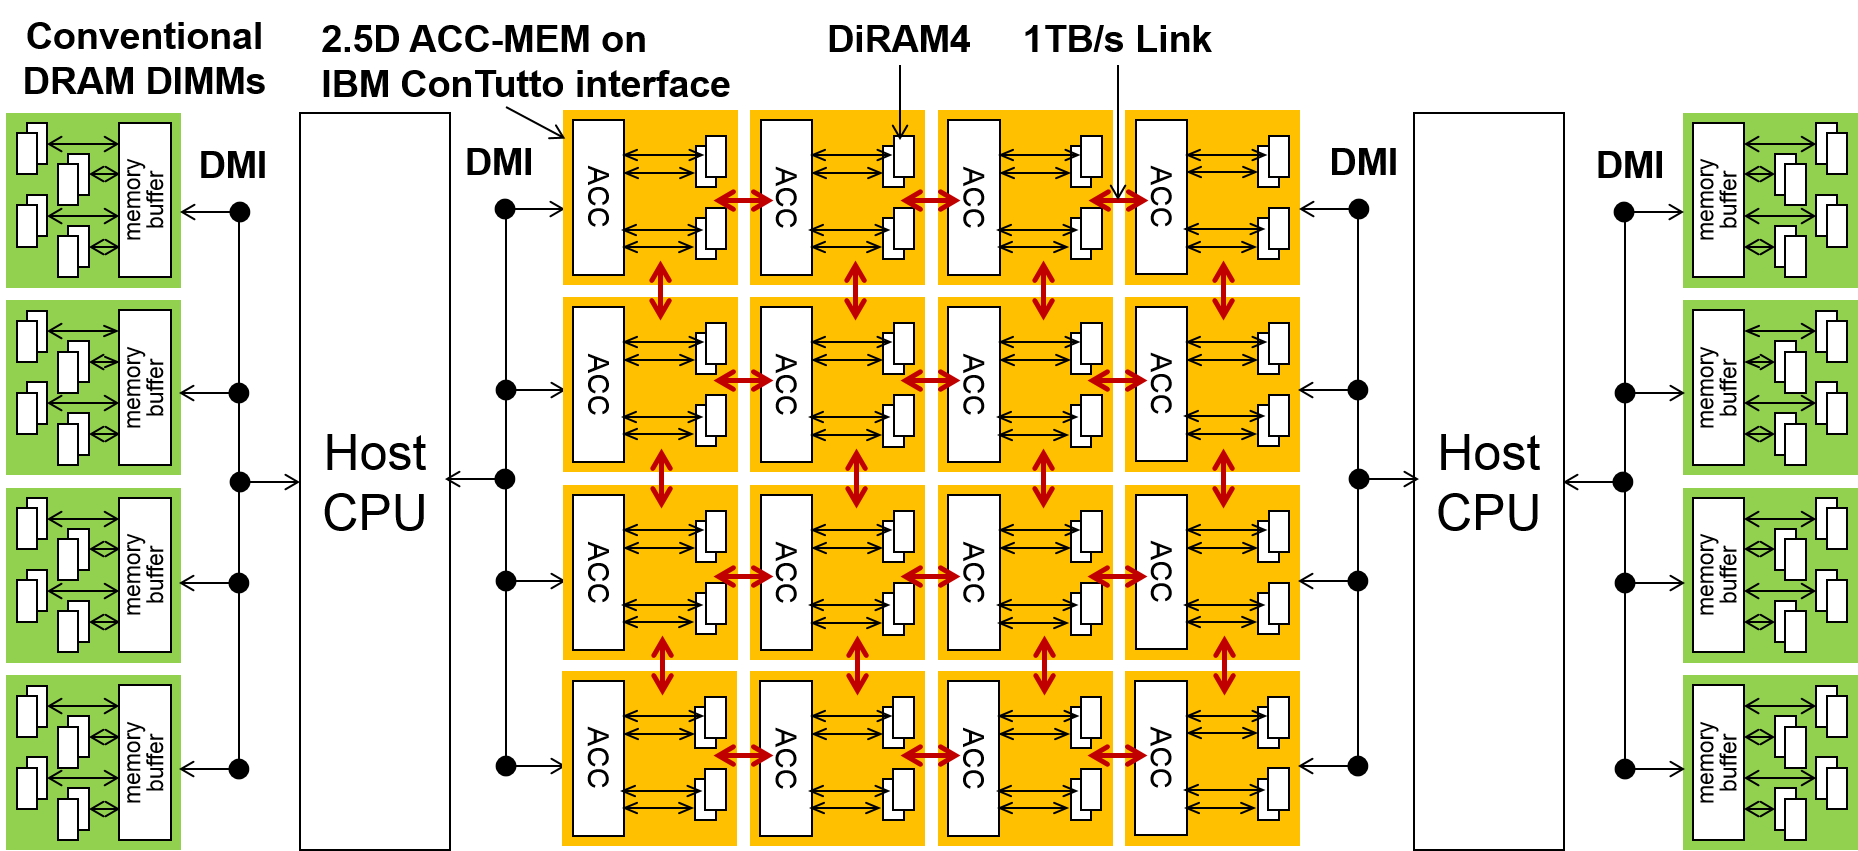
\includegraphics[width=1.0\linewidth]{fig/arch.png}
\caption{GAMA System Architecture}
\label{fig:arch}
\end{figure}
 


\begin{comment}

%the memory channel provides the highest bandwidth with the lowest latency amongst off-chip communication interfaces in contemporary computer systems.

 
 %Specifically,  a DiRAM4 die provides the same aggregate bandwidth as HBM2, but it provides 4X more channels than HBM2 where each channel supports only a quarter of the width of HBM2. We believe that DiRAM4 design is better suited for graph analytics where multiple accesses are made to random 


High bandwidth memory (HBM) and hybrid memory cube (HMC) used for recent PIM architectures can provide high bandwidth only for sequential, regular memory accesses. In contrast, graph analytics require efficient support for irregular and small granularity memory accesses. We tackle this problem by adopting a recent DiRAM4 3D Memory from Tezzaron and architecting on-chip caches and a custom memory controller to efficiently support small granularity irregular memory accesses. 
Specifically, DiRAM4 provides the same aggregate bandwidth as HBM2, but it provides 4X more (but narrower) channels than HBM2

.  The tiled architecture is built  

In this project, we envision to develop a PIM system depicted in Figure~\ref{fig:arch}. 
Overall, the system consists of a 16-node accelerator-memory (AM) cluster and IBM POWER8-based host systems.
An AM cluster is comprised of 16 nodes (packages) connected by our power-efficient high-bandwidth chip-to-chip links in a mesh style. 
One accelerator (ACC) and four 8GB DiRAM4 dies will constitute a PIM package with 4TB/s aggregate in-package bandwidth. 
%Our ACC die will integrate 16 ACCs with our custom eDRAM-based large shared and SRAM-based private on-chip cache, a 16$\times$16 crossbar, and a network interface (NI) to support chip-to-chip communications.

\begin{wrapfigure}{r}[0pt]{0.6\textwidth}
\center
%\vspace{-8ex}
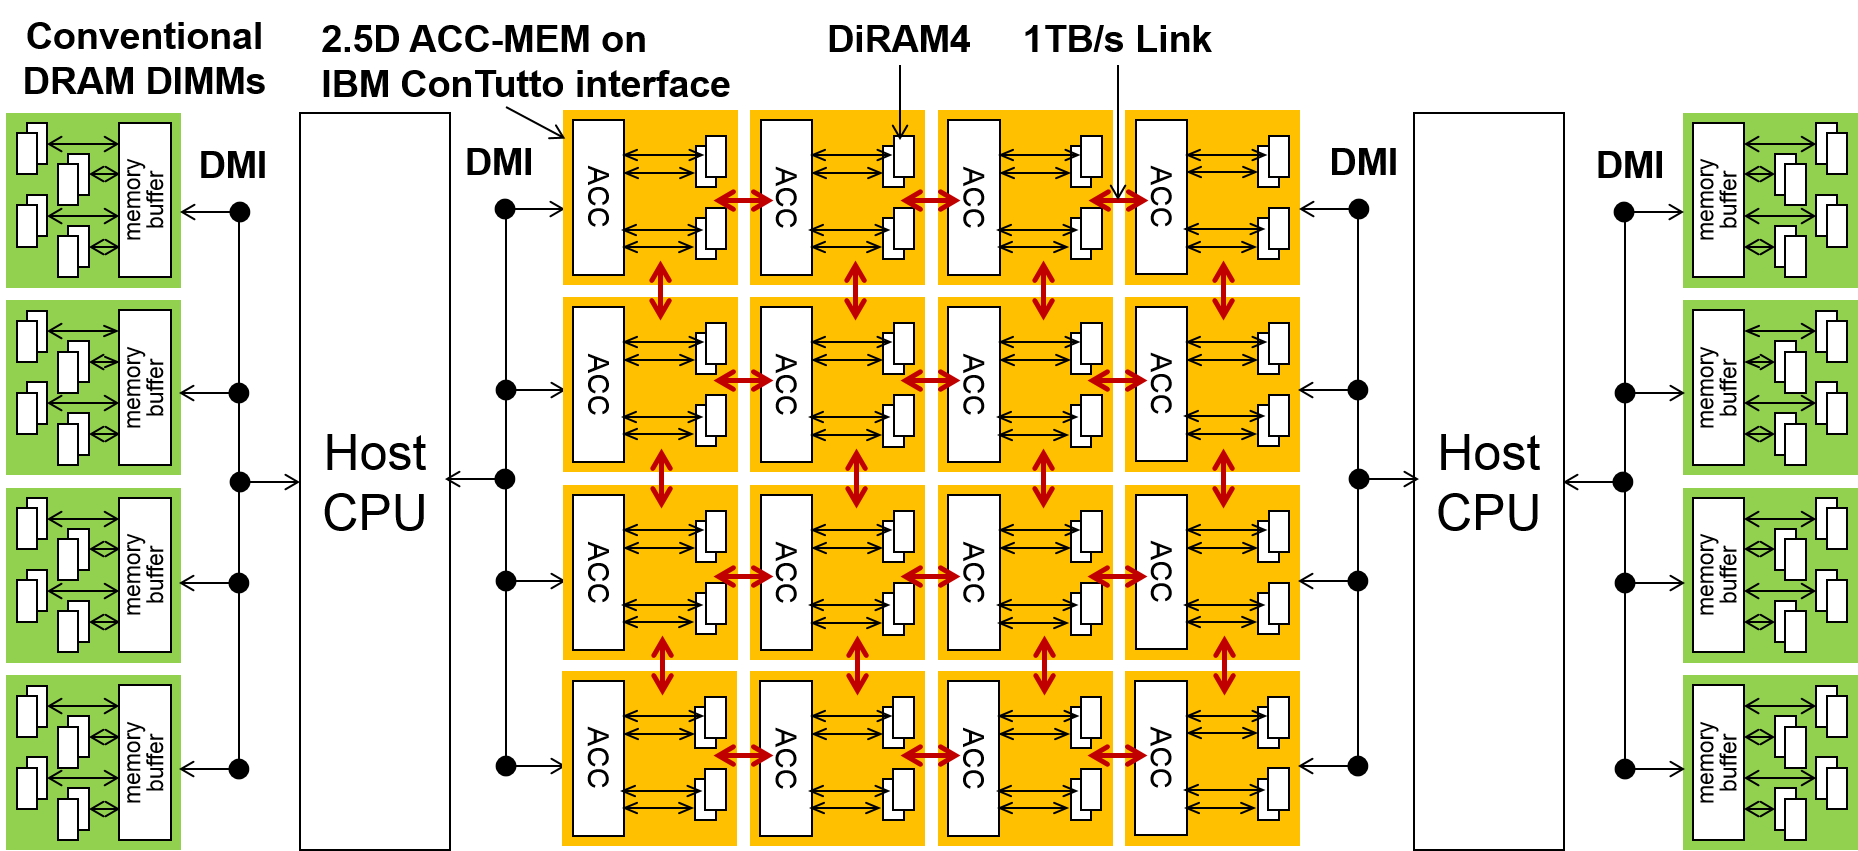
\includegraphics[width=1.0\linewidth]{./fig/arch.png}
\caption{The overall architecture of an Accelerator-Memory HIVE.}
\label{fig:arch}
\end{wrapfigure}

In the proposed PIM system, we propose to connect each AM packages to a memory channel of a host CPU providing 8 memory channels;
the memory channel provides the highest bandwidth with the lowest latency amongst off-chip communication interfaces in contemporary computer systems.
A IBM's ConTutto facilitates the interface between an AM package and the IBM's proprietary memory interface (DMI).
The memory space associated with the AM cluster is a non-cacheable region to eliminate the need for managing cache coherence between caches of the host systems and the AM HIVE.
The host system allocates the memory space of the AM cluster as a sinlge, continuous, and large physical memory segment which is preferred by big-data applications~\footnote{}.
ACCs are memory-mapped to part of the non-cacheable regions (as other I/O devices).

% Some notes
% We need a custom POWER8 board
\end{comment}


\subsection{ACC Architecture}
\label{sec:processing}
\noindent
The basic building block of the GAMA accelerator (Fig.~\ref{fig:arch}(b)) is the GAMA core,
RISC-V processor with tightly coupled with an 8-lane acceleration engine to efficiently accelerate sparse matrix operations (Fig.~\ref{fig:arch}(c)).
The core is architected to provide 16GOPs at 34mW and the estimated area is 0.5mm$^2$.
We will first describe the microarchitecture of the GAMA core, and then describe the overall architecture of the GAMA accelerator.


It has been shown that a wide range of graph algorithms can be implemented by a general case of matrix multiply \textbf{C} = \textbf{A} \textit{f}().\textit{g}() \textbf{B} 
For example, a matrix-vector multiply (i.e., \textbf{C} = \textbf{A} +.$\times$ \textbf{B}) represents an one-hop BFS 
where \textbf{A} is a $N \times N$ connectivity matrix, \textbf{B} is a $1 \times N$ vector of the starting node, 
\textit{g}($i$, $j$) returns $a_{i,j} \times b_{j}$ and \textit{f}($i$) returns $\sum_{j=1}^{N}$ \textit{g}($i$,$j$).


As large graphs are often represented by very sparse matrices, compressed formats are widely used to efficiently store the matrices in terms of storage size.
However, this complicates matrix operations and requires random/irregular memory accesses especially for constructing \textbf{C} in a compressed format on the fly (i.e., merging operations).
After carefully analyzing the state-of-the-art DCSC and DCSR formats and matrix multiplication algorithms based on these formats, 
we propose the GAMA core microarchitecture depicted in Fig.~\ref{fig:arch}(c).
That is, an 8-lane engine to accelerate sparse matrix operations is tightly coupled with a RISC-V processor.


In this microarchitecture, we first aim to avoid storing \textbf{A} and \textbf{B} in multiple formats, which often simplifies the accesses of specific non-zero values (NZVs) of \textbf{A} and \textbf{B} for matrix operations.
Our microarchitecture can handle both row- and colum-major formats, but suppose both \textbf{A} and \textbf{B} are stored in DCSC or similar column-major format for the brevity of description.
In such a format, NZVs in a given column are already sorted in row order and stored in an array structure sequentially. 
To stage NZVs with their row indices from both \textbf{A} and \textbf{B} for parallel operations, we propose A- and B-column buffers. 
Each buffer consists of one or more 64-byte entries, each of which can be loaded by one special load instruction (\texttt{LD64B}) that we will implement in the RISC-V processor. 
Note that \texttt{LD64B} will bypass L1D cache and directly access the GAMA main memory, as these buffers serve as cache for NZVs and row indices from \textbf{A} and \textbf{B}.
A buffer entry stores 8 pairs of a value and its row index from a column of a matrix (Fig.~\ref{fig:arch});
we assume that the number of NZVs in a column is still much larger than that of 8 in an acceleration engine in large matrices of project's interest, and thus
the corresponding column address for all 8 pairs is stored in the register file of the RISC-V processor.


Consider the first pair in ``B-column buffer'' in Fig.~\ref{fig:arch}(c).
The row index determines the column index of \textbf{A} stored in DCSC or similar column major format.
For a given column, the column-major sparse matrix format allows us to easily retrieve the starting address and the number of NZVs sequentially stored in the array. 
After the processor determines the starting address and the number of NZVs of the corresponding column, 
it also loads 8 pairs of a value and its row index in an entry of ``A-column buffer'' by executing a \texttt{LD64B}.


As depicted, there are 8 ALUs for \textit{g}(), and the value in the first pair of the B-column buffer is broadcast to all 8 ALUs as one of the operands in each ALU.
The 8 values in the first entry of the A-column buffer are fed to the 8 ALUs as the other operand for each ALU.
We will use ALUs supporting single-precision floating-point multiply-add operations.
However, all the NZVs will be ``1'' and a multiplication can be replaced with a ``AND'' operation for graph traversing problems.
In such a case, we propose to power-gate the floating-point unit in the ALU and run the core at higher frequency than 2GHz, as
AND operations consume much less power than floating-point operations and less contrained by power and thermal issues. 


The 8 computed results with the corresponding 8 row indices from the first entry of A-column buffer will be applied to 
the ``parallel memory access unit'' 
,
the column index of values in B-column buffer, and the starting address of the heap associated with the column index of B-column buffer.
The heap is used to construct \textbf{C} (cf. A. Buluc, et al., ``On the Representation and Multiplication of Hypersparse Matrices,'' IDPDS, 2008)
As the access pattern of the heap is very random, these 8 values with random addresses will be stored to our elastic L1D cache (cf. Sec.~\ref{sec:memory:on-chip}) with 8 banks to support 8 concurrent accesses to 8 different random addresses.
Moreover, we will use the ALUs support three-operand computaions such as multiply-add to efficiently support the accumulation of values computed by 8 values to the corresponding values of \textbf{C} stored in the heap.


After all the NZVs of column ``1'' of \textbf{A} is consumed in Fig.~\ref{fig:arch}(c), 
the B-column buffer acting like a FIFO buffer makes the second entry the first one, and the processor brings the values and row indices of column ``11'' of \textbf{A}. 
Also, the row indices sotred in B-column buffer can be used for prefetching NZVs and the corresponding row indices of the next columns of \textbf{A} to A-column buffer.


The RISC-V processor has 4KB IL1 and 32KB 8-bank DL1 caches.
The processor will be enhanced to efficiently perform various management tasks for the acceleration engine such as:
calculating the starting memory addresses of arrays containing NZVs and their associated row values of columns; and
controlling the data-flow of the acceleration engin for merging operations for constructing \textbf{C} through the heap.
 

%Then it issues an instruction that brings 64 bytes containing 8 pairs of row index and associated value and store them . 
%is to process elements from a (subset of) row of \textbf{A} and a (subset of) column of \textbf{B} (Fig.~\ref{fig:acc-arch}(b)).
%This is advantageous for a given \textit{f}($i$) to efficiently operate on \textbf{g}($i$, $j$).
%For efficient execution of complex \textbf{g}() and \textbf{f}(), we propose to use 


The architecture of a GAMA accelerator is composed of four MIMD clusters, and the cluster architecture is depicted in Figure~\ref{fig:arch}(b).
A cluster consists of 16 cores operating at 2GHz and connected to a special 512KB eDRAM-based L2 cache (cf. Sec.~\ref{sec:memory:on-chip}) and a 16GBps on-chip interconnect between them. 
An eDRAM L2 cache can be connected to one of 16 DiRAM4 memory controllers, each of which is connected to a 64-bit (16GBps) DiRAM4 memory channel, through switches.
Moreoever, a core can send a memory request to a port of the OpenCAP link consisting of 16 ports and providing 256GBps aggregate bandwidth, as well as network on-chip (NOC) interconnects to three other clusters.  
%which are connected to each other through on-chip network.


\begin{comment}
\noindent
\textbf{Coarse-Grained Reconfigurable Processing Engine:} 
To efficiently execute graph primitives, we aim to architect the CGR-Core with a coarse-grain reconfigurable (CGR) array of execution units. 
This architecture based on a spatial data-flow architecture can significantly reduce the overhead of instruction fetches and data transfers within an accelerator, as many operations for a complex graph primitive function can be executed by a single (macro) instruction and a few registerfile and/or cache accesses. 
Furthermore, for streaming graph analytics, it is very inefficient to apply computations and changes to individual vertices as they arrive. 
We propose the update buffer to allow CGR-Core to bulk commit messages bound for (or coming from) multiple vertices in a single phase.
\end{comment}



\begin{comment}
\noindent
\textbf{Trailblazer:} 
One of the unique properties of graph algorithms is that all vertices perform the same computation (with some limited control flow support). 
Hence, the execution behavior of future vertex computations can be easily inferred from current vertex computations. 
We will use the notion of trailblazing where some of the vertex computation tasks are closely monitored. 
During trail blazing various microarchitectural events are monitored, such as memory bandwidth, branch behavior patterns and affinity of communication between different vertices. 
We hypothesize that there are pairs of vertices that exhibit dominant communication patterns which can be inferred from trail blazing. 
We will use the knowledge from trailblazing to potentially co-locate affine vertices to the same compute node. 
The notion of trail blazing was used for prefetching irregular data in CPUs, but we plan to apply similar principle for managing vertex computations.

%which is a 16-wide SIMD pipeline that is optimized by vector multiply-accumulate operations. 
%Each core is provisioned with \emph{Elastic} L1D cache.  

%32 corelets are placed on a single die and share a single large L2 cache designed using eDRAM. The L2 cache is then backed up by 4X8GB DiRAM4 memory modules. DiRAM4 is a die-stacked DRAM die that is provided by Tezzaron (one of our service providers in this project). The 32 corelets are 2.5D stacked with DiRAM4. This entire package is called a GAMA tile. We will integrate 16 GAMA tiles to create the whole GAMA accelerator system. 16 GAMA tiles are interconnected  using our custom-designed 1Tbps inter-tile interface. The GAMA system is interfaced with IBM Power8-based host system using OpenCAPI interface. 
%At each layer of the above design we propose several innovative ideas. At the corelet layer we propose to design specialized address mapping engines that translate the sparse matrix indices to generate the row/column index of matrix elements based on the underlying sparse matrix format. While the 32 GAMA corelets can do MIMD computations they can  be dynamically reconfigured to execute a single instruction across a very wide vector range when accesses are highly sequential.  The elastic  cache attached to each corelet is architected to support both dense/sequential and sparse/random accesses to a matrix. The elastic cache is a low-overhead cache organization that supports variable width cache lines to improve cache usage efficiency.  
% The unique aspect of DiRAM4 memory, compared to other competing memories such as high bandwidth memory, is that each DiRAM4 die supports more channels per die, but uses narrow width channels. Such a design is well suited for graph workloads that need narrow width memory level parallelism. The narrow width channels can be reconfigured to create a single wide width channel to support dense matrices. The memory layer itself is made semantically aware of the matrix structure and its preferred lay out and access patterns in memory. The semantic awareness comes from application provided hints that are conveyed to the memory controller through APIs. Since graphs that are spread over multiple tiles demand high bandwidth inter-tile access. High-bandwidth links  posing power, thermal, and signal integrity challenges.  We tackle this challenge with various charge-based and injection-locking techniques for high-speed links. The scalability of parallel graph algorithms will be improved by enabling barrier elision hardware that can be used by the application developer to tradeoff accuracy with latency. We provide an in-depth visibility to software to monitor changes to the graph structure and take action to deal with potential load imbalances.  

%32 corelets are placed on a single die and share a single large L2 cache designed using eDRAM. The L2 cache is then backed up by 4X8GB DiRAM4 memory modules. DiRAM4 is a die-stacked DRAM die that is provided by Tezzaron (one of our service providers in this project). The 32 corelets are 2.5D stacked with DiRAM4. This entire package is called a GAMA tile. We will integrate 16 GAMA tiles to create the whole GAMA accelerator system. 16 GAMA tiles are interconnected  using our custom-designed 1Tbps inter-tile interface. The GAMA system is interfaced with IBM Power8-based host system using OpenCAPI interface. 
%At each layer of the above design we propose several innovative ideas. At the corelet layer we propose to design specialized address mapping engines that translate the sparse matrix indices to generate the row/column index of matrix elements based on the underlying sparse matrix format. While the 32 GAMA corelets can do MIMD computations they can  be dynamically reconfigured to execute a single instruction across a very wide vector range when accesses are highly sequential.  The elastic  cache attached to each corelet is architected to support both dense/sequential and sparse/random accesses to a matrix. The elastic cache is a low-overhead cache organization that supports variable width cache lines to improve cache usage efficiency.  
% The unique aspect of DiRAM4 memory, compared to other competing memories such as high bandwidth memory, is that each DiRAM4 die supports more channels per die, but uses narrow width channels. Such a design is well suited for graph workloads that need narrow width memory level parallelism. The narrow width channels can be reconfigured to create a single wide width channel to support dense matrices. The memory layer itself is made semantically aware of the matrix structure and its preferred lay out and access patterns in memory. The semantic awareness comes from application provided hints that are conveyed to the memory controller through APIs. Since graphs that are spread over multiple tiles demand high bandwidth inter-tile access. High-bandwidth links  posing power, thermal, and signal integrity challenges.  We tackle this challenge with various charge-based and injection-locking techniques for high-speed links. The scalability of parallel graph algorithms will be improved by enabling barrier elision hardware that can be used by the application developer to tradeoff accuracy with latency. We provide an in-depth visibility to software to monitor changes to the graph structure and take action to deal with potential load imbalances.  

%%%
%%% An accelerator architecture and processor pipeline which supports the processing of identified graph primitives in a native matrix format.
%%%
%
% Doing some research on ``An accelerator architecture and processor pipeline which supports the processing of identified graph primitives in a native matrix format.'' in BAA
% I think we should propose a processing core that can perform well for sparse matrix computations. 
% Also look at ``Standards for Graph Algorithm Primitives.'' This shows that graph algorithms such as BFS can be done with sparse matrix multiplications.
% That is, we should propose a processing pipeline that can efficiently do sparse matrix.

In this project, we aim to architect processor pipeline that can efficient support more general cases of sparse matrix multiply (Fig.~\ref{fig:acc-arch}).
Toward this goal, we envision an MIMD architecture where 16 processors constitute a cluster.
A cluster has two 16-bank L1 data caches to cache \textbf{A} and \textbf{B} (denoted by A- and B-cache), respectively.
The address space partitioning set by a programmer.
Depending on a given compressed format, either A or B will have more random accesses (e.g., B for CSR).
In this way, we can better preserve locality of one of the caches.
Supposing \textbf{A} is stored in CSR format, 
The processors and A-/B-caches are connected by two 16$\times$16 crossbars (denoted by A- and B-xbars), respectively.
Each processor is an in-order processor with a coarse-grain reconfigurable (CGR) execution unit.

supporting single (complex) operation per cyle in terms of its throughput  
\end{comment}



\subsection{Memory Sub-system Architecture}
\label{sec:memory}
%%% A chip (or possibly multichip) architecture that support the easy movement of data from
%%% memory or IOs to the accelerators based on an ``identified data flow model''. Emphasis
%%% should be on redefining cache based architectures so that they address both sparse and
%%% dense data sets. Integration of the processor and memory architecture may be necessary.


%%% An external memory controller which is designed to ensure efficient us of the identified
%%% ``data mapping tools''. The controller should be able to efficiently handle random as well as
%%% sequential memory accesses. Every effort should be made to minimize the size of the data
%%% access to avoid the need to pad memory. The use of advanced memory technology may
%%% be necessary

%%% How will you design a memory controller to take advantage of the data maps?
%%% The key to efficient processing of large scale graph analytics is to ensure the locality of
%%% information. The less you have to move the data, the more efficient the computation from both a
%%% power and performance perspective. The memory controller needs to exploit locality regardless
%%% of whether the dataset is sparse or dense.

\noindent
Our preliminary study~\cite{Xu2014, luo2010effective, kim2015compiler, kim2015locality} show that the memory bandwidth utilization is very low for many graph algorithms.
Graph algorithms often require random/sparse memory accesses, whereas the memory hierarchy is optimized only for sequential/dense memory accesses.
We must re-design the entire memory hierarchy to effectively support both random/sparse and sequential/dense memory accesses.
That is, optimizing either on-chip caches or off-chip memory alone is ineffective.
Thus, we propose to architect the GAMA memory system, consisting of (1) a private L1 cache for each GAMA core; (2) shared spatially-temporally boosted eDRAM L2 caches across all the cores within a GAMA tile; and (3) 32GB of DiRAM4 with a custom memory controller, to efficiently support random/sparse and sequential/dense memory accesses.
More specifically, it will be built on circuit/architecture techniques and a soon-to-be-released DRAM technology and will achieve the target 90\% utilization of memory bandwidth. 


\subsubsection{On-Chip Cache Architecture} 
\label{sec:memory:on-chip}
\noindent
\textbf{L1 cache.}
We propose elastic cache architecture to efficiently support both narrow- and wide-width memory accesses from multiple non-contiguous memory locations to co-reside in a single 64-byte cache line. 
Specifically, we introduce a concept of chunk tags to store tags for narrow-width data blocks (e.g., 4-, 8-, or 16-byte byte blocks) along with a conventional tag (referred to as common tag) for each 64-byte cache line (see Fig.~\ref{fig:elastic-cache}(a) fror how the chunk and common tags are architected).  Chunk tags add only a small storage overhead. 
Elastic cache allows us to efficiently use cache lines for storing narrow-width data blocks from non-contiguous addresses (i.e. the heap memory accesses to construct \textbf{C} on the fly, 
which may be seen in sparse matrices, as well as a 64-byte contiguous blocks that may be seen in dense matrices without significant cache reorganization. 
Note that just adopting narrow cache lines is not efficient to handle sequential memory requests for dense datasets according to our experiments.
Our preliminary study shows this architecture applied to L1 caches alone in  a traditional GPU architecture improves the performance by more than 2$\times$ for SPMV (sparse matrix-vector muliply).
We expect that the performance can be further improved when the architecture is also applied to large L2 cache.


%Note that just adopting narrow cache lines is not efficient to handle sequential memory requests for dense datasets according to our experiments.
%Figure~\ref{fig:elastic-cache-flow} describes the access flow of the proposed \texttt{Elastic-Cache}. 
%Note that we will employ the proposed \texttt{Elastic-Cache} architecture for both private SRAM-based L1 and shared eDRAM-based L2 caches.

\begin{comment}
\begin{wrapfigure}{r}[0pt]{0.4\textwidth}
\center
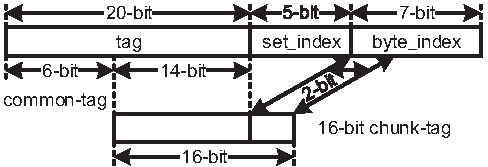
\includegraphics[width=1.0\linewidth]{./fig/chunk_tag_16bit-eps-converted-to.pdf}
%\caption{The chunk and common tags to support both narrow- and wide-width on-chip cache accesses for a 4-way 16KB cache.}
\caption{The chunk and common tags to support elastic cache accesses for a 4-way 16KB cache.}
\label{fig:elastic-cache}
\end{wrapfigure}
\end{comment}


Considering our core architecture with a 8-lane engine (cf. Sec.~\ref{sec:processing}), 
we will architect the elastic L1 cache with 8 banks. 
Each bank is a 4KB direct-map cache with 4 victim entries and provides 8 bytes per cycle (i.e., total 64 bytes per cycle).
This architecture is preferrable, as the 8-lane SIMD engine with the address generation logic in Fig.~\ref{fig:arch}(c) can simultaneously request 8 memory accesses to different addresses for the heap memory accesses.
%The connection between an elastic L1 cache and a corelet is described in Section~\ref{sec:processing}.

\begin{figure}
\center
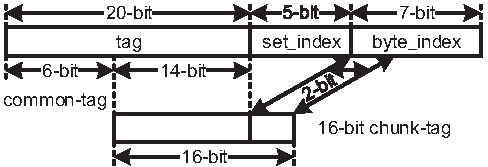
\includegraphics[width=0.3\linewidth]{./fig/chunk_tag_16bit-eps-converted-to.pdf}
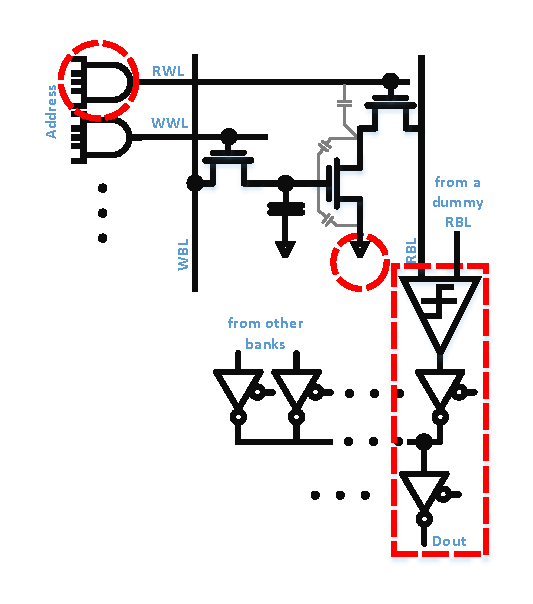
\includegraphics[width=0.2\linewidth]{./fig/boosting.pdf}
%\caption{The chunk and common tags to support both narrow- and wide-width on-chip cache accesses for a 4-way 16KB cache.}
\caption{(a)Elastic cache: chunk and common tag architecture (b) Boosting scheme for 3T eDRAM bitcells}
\label{fig:elastic-cache}
\end{figure}

\begin{comment}
\begin{wrapfigure}{r}[0pt]{0.35\textwidth}
\center
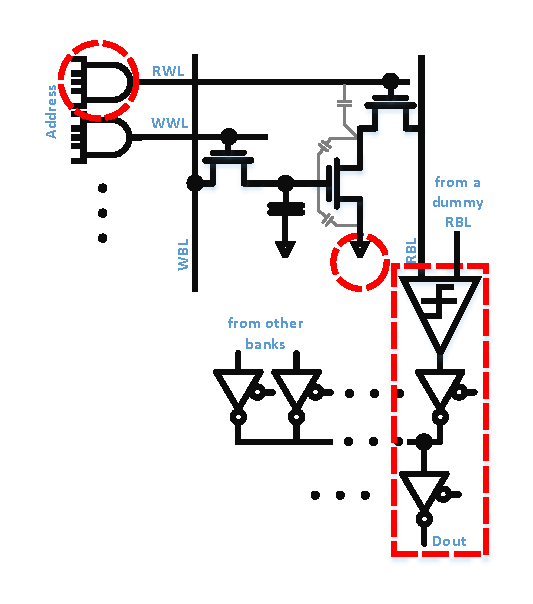
\includegraphics[width=2.4in, trim=20 20 10 50]{./fig/boosting.pdf}
\caption{A boosting scheme for the cache with 3T eDRAM bitcells.} 
%Red dashed outlines highlight the portions receiving boosting/underdriving. It is critical to protect dynamic nodes from coupling noises of boosting via parasitic capacitors (gray).}
\label{fig:boosting}
\end{wrapfigure}
\end{comment}

%\vspace{3pt}
\noindent
\textbf{L2 cache.}
The L2 cache is shared amongst 32 GAMA cores and is implemented with eDRAM and the same elastic cache architecture as L1 cache. 
In implementing eDRAM cache, we aim to overcome relatively long latency of accessing eDRAM cache compared with SRAM cache. 
%minimize latency %and support \texttt{Elastic-Cache} data access. 
%In the eDRAM based L2, it is particularly critical to 
%In this project, %building upon our recent work on low-energy and compact memory-based FFT core\footnote{ISSCC'17 submitted}, 
We will apply a dynamic fine-grained spatial-temporal voltage boosting technique only on the peripheral circuits (address decoders, multiplexers/demultiplexers, and interconnect buffers), but not bitcells. 
This boosting technique is synergistic with the elastic cache architecture and beneficial for graph algorithms that often need to access a small subset of a large cache line without dissipating excessive power. 
We will explore voltage boosting in a temporarily and spatially fine-grained fashion for improving access latency and throughput (cf. Fig.~\ref{fig:elastic-cache}(b)). 
We will also effectively gate or use low supply voltage (e.g., 0.6V or lower) for the circuits that are not involved in accessing the demand data, making them serve as thermal buffers. 
%This way, we expect to significantly improve latency still under the thermal limit. 
Assuming 0.5V threshold voltage ($V_T$), 
%\footnote{High $V_T$ is common in embedded memory for suppressing leakage}
boosting from 0.8V to 1.4V can increase the overdrive level ($V_{DD}$-$V_T$) from 0.3V to 0.9V, improving latency and throughput by at least 3$\times$. 
%The low $V_{DD}$ used in the rest of cache circuits can save a significant amount of leakage energy dissipation. 
By exploiting this latency improvement, we will explore to make the cache systems to perform multiple fine-grained data accesses (in serial by default but in parallel if data are in the multiple banks) and pack and send them back to the pipeline of a core. 
To enable such voltage boosting in a short time period without exceeding the power/thermal limit, 
we will explore circuit innovations from our own prior works~\cite{yang2015compact,  Doyun2017, kim2014analysis}, such as precise thermal monitoring to stop voltage overdrive that may occur with higher temperature, and sub-cycle voltage boosting through decoupling capacitor design and in-situ error monitoring.


\begin{comment}
To enable such voltage boosting, we need to meet two requirements.  First, we need to boost voltage in a fraction of cycle time. 
This can be achieved first by having strong power-grid for boosted voltage, together with a good amount of decoupling capacitors circuits. 
Still, the power grid, due to the sub-nanosecond transient change, can undergo a non-negligible amount of voltage integrity degradation (i.e., droops, overshoot, and ripples). 
%Over-designing power grids and decoupling capacitors can incur significant area and energy overhead. 
Our approach to this challenge is to apply techniques that tolerate such problems in power grids through in-situ error detection and correction (EDAC), as EDAC can detect and correct timing errors from supply voltage droop without over-design and the worst-case margin. Specifically, we will develop an EDAC technique that primarily focuses on detecting errors and allowing instruction replays to deal with error correction.

Second, we need small and precise thermal monitoring systems to stop voltage overdrive if temperature rises above a temperature limit. 
Note that existing state-of-the-art in on-chip thermal monitoring, however, have been limited due to sensor circuits that are too invasive in terms of size ($>$ a few thousand $\mu m^2$ per sensor) and voltage-scalability (requiring $>$ 1V). 
This limitation prevents sensors from being placed closely to digital hotspots. 
In this project, we will create improved thermal monitoring systems for embedded memory based on our recent thermal sensor designs that achieves about two orders of magnitude more compact (30 $\mu m^2$ per sensor), comparably or more accurate ($\pm 1.1^oC$ 3-$\sigma$ error), and voltage scalable down to 0.4V  \footnote{T. Yang et al., ``Ultra-compact and Voltage-Scalable Temperature Sensor Design for Dense Dynamic Thermal Management Techniques,'' \textit{IEEE Journal of Solid-State Circuits (JSSC)}, 2015; S. Kim et al., ``A $30.1\mu m^{2}$, $\pm 1.1^{o}C$-$3\sigma$-Error, 0.4-to-1.0V Temperature Sensor based on Direct Threshold-Voltage Sensing for Dense On-Chip Thermal Monitoring,'' \textit{IEEE Custom Integrated Circuits Conference (CICC)}, 2015}. 
%By placing such sensors closely to estimated hotspots, we anticipate to achieve high accuracy in thermal monitoring, which will allow us to use voltage boosting longer and more frequently without pessimistic throttling. 
Furthermore in eDRAM caches, accurate thermal sensing will be used to adaptively change the refresh cycles, saving energy and increasing access availability. 
\end{comment}


\subsubsection{Off-Chip Memory Architecture} 
\label{sec:memory:off-chip}
\noindent
\textbf{Memory technology.} 
We will use  Tezzaron's DiRAM4 for the main memory of each GAMA tile.  
Each DiRAM4 die provides 8GB capacity with 64$\times$32-bit ports (total 2048 I/O pins) with 1TB/s bandwidth. 
HBM2 is expected to provide the same bandwidth as DiRAM4, but we choose DiRAM4 because it provides narrower but more memory channels than HBM2 (16$\times$128-bit channels). 
We believe that DiRAM is more advantageous than HBM2 for graph algorithms that generate random/sparse memory accesses. 
Each tile integrates 4$\times$8GB DiRAM modules and thus there is a total of 4TBps internal memory bandwidth between the GAMA core and the main memory within each tile. 


\vspace{3pt}
\noindent
\textbf{Memory controller.} 
We propose a memory controller architecture supporting dynamic memory channel reconfigurations to effectively support both random/sparse and sequential/dense accesses.
By default the GAMA main memory system starts with many narrow memory channels to efficiently service random/sparse memory accesses.
However, %after the current or expected memory access patterns is determined based on a data map (cf. ``Data placement and memory map''),
64 memory channels can be dynamically chained to form wider logical memory channels, each with a larger memory queue for efficient sequential/dense memory accesses.
That is, multiple small memory requests can be merged (coalesced) into one single memory request, allowing more efficient utilization of the memory scheduling queue.
%When narrow memory channels are fused into a wide (logical) memory channel, 
%we have more memory scheduling queue entries in a logical memory controller.
%These two aspects improve the utilization of both command/address and data buses for sequential/dense memory accesses.


To dynamically configure the memory channels, we exploit the information from the provided memory map stored for each matrix (cf. ``\textbf{Data placement and memory map}'').
%and large front-end memory queues. 
The datamap enables the memory controller to infer how consecutive elements of a row or column (irrespective of whether the matrix is dense or sparse) are laid out. 
The front-end memory queue buffers the requests from cores across the entire GAMA system, as all GAMA tiles see a globally shared address space (cf. \textbf{``Memory model''}). 
The memory queue monitors the requests from multiple cores and determines all the requests that are bound to a given bank or channel. 
It will then pull all the data from a single channel that may satisfy multiple requests from a core.  


To support a large memory queue for efficient coalescing, 
we adopt a two-stage memory queue structure with a large number of entries in the front-end queue. 
The memory controller with this proposed  memory queue may decide to delay requests for a short interval that does not affect the utilization of cores and memory channels. 
%As each GAMA tile computes over a slice of compressed vectors (or a slice of a row or column in a dense matrix), 
%we expect that memory requests from different cores within each tile may exhibit spatial locality. 
%Even sparse matrix representations will exhibit strong spatial locality across row or column values that are used in a given matrix operation.  
%Thus the front-end memory queue buffers requests and extracts spatial locality by coalescing memory requests. 
This allows the front-end memory queue buffers requests and extracts more spatial locality by coalescing memory requests. 
%Note that the traditional memory queues cannot be large because they rely on CAM.
%Instead of CAM-based memory queue, we aim to architect the large memory queue using a structure like set-associative cache, where entries are indexed by memory request address ranges to confirm the full matching after comparing the tags associated with the index.
%A list structure associated with the memory queue keeps track of valid entries in the cache-like structure based on a scheduling policy and sends the entries to the back-end memory queues associated with each DRAM bank.

\vspace{3pt}
\noindent
\textbf{Memory model.} 
The GAMA system will adopt a distributed shared memory model with non-uniform memory access latency. 
Hence, all the 16 GAMA tiles will share the address space. 
The programer uses the OpenCAPI protocol to launch a sparse matrix operation on the GAMA accelerator. 
OpenCAPI reduces the overhead and complexity of sharing the main memory and maintaining cache coherence amongst host CPUs and accelerators.
Specifically, OpenCAPI provides the libcxl library for initiating accelerator launch and memory management APIs, such as $cxl\_afu\_open\_dev$ to open the accelerator and $cxl\_afu\_attach$ to start the accelerator. 
The data for the accelerator is placed in a work element descriptor (WED) and is passed as a pointer to GAMA. 
The accelerator and host can seamlessly share the same virtual memory space. 

\begin{comment}
\vspace{3pt}
\noindent
\textbf{Data placement.} 
%Each 128MB data slice may be further interleaved in various banks and channels within each tile.  
Given the criticality of memory latency and bandwidth to graph processing, 
we will provide several higher-level software APIs to allow the application developer or compilers (T2 thrust perfomers) to provide semantic information about matrix representations laid out in memory. 
For instance, the programmer may explicitly tag the column pointer, row index and value vectors (for compressed column representation). 
This information will be used by the memory system to determine how to layout these arrays (bank interleaving and distribution across memory channels) in memory and also to generate bank and channel access commands for each vector appropriately. 
% intermediate matrices and vectors that may be generated  may also be tagged by the programmer to indicate how they are being stored (doubly compressed column or row etc.,).  %For instance, in centrality analysis using all pairs shortest paths approach the shortest paths for each pair are stored as intermediate results that will be used in the final reduction process to extract the central vertex.  Each matrix or vector's  physical address to appropriate bank and channel activation sequence.
%Appropriate interleaving of data across a large number of channels is critical for enabling parallel access. 
%If requests from multiple GAMA corelets can be routed to different channels then their requests can be satisfied in parallel. 
Depending on the sparse matrix representation some data structures may see sequential accesses to large blocks while other structures may encounter mostly random accesses. For instance, in a compressed column  representation the column pointer vector is randomly accessed to select a given column (for instance, in a BFS the starting vertex column) and then the value in column pointer is used as index into row index  vector and value vector. The row index and value vectors are scanned together to reconstruct the column. Hence it is best to put the row index vector and value vector on different channels which can be concurrently accessed to accelerate the column reconstruction.  

For dense matrices we expect the programmer to use the software API to provide hints to the hardware whether a matrix is predominantly accessed column-wise or row-wise in the next computation phase. 
These hints can be updated at various computation phases in a kernel. The hardware uses this information to decide on an appropriate matrix layout in memory. 

%MURALI:SHOULD WE INCLUDE THIS LEVEL OF DETAILS?
\end{comment}

\vspace{3pt}
\noindent
\textbf{Data placement and memory datamap.} 
By default the data is interleaved across the tiles at the granularity of 128MB. 
This interleaving allows significant amount of contiguous matrix data to be placed per each tile, while at the same time allowing a large matrix to be mapped across multiple tiles to improve memory parallelism.   
Once the data (either sparse or dense matrix) is laid out in each GAMA tile's memory, 
a metadata table (or datamap) will be generated to indicate the row and columns ranges stored at each tile for a given matrix.   

The datamap also stores the  approximate number of NZVs in each row and column of a matrix in a distributed manner across multiple tiles. 
As described later, the sparsity information is used to improve load balancing.     
The metadata may also store finer-granularity information such as the channel and bank interleaving information for rows and columns. 
This metadata information will be used to enable simple optimizations such as gating bank activations 
when a given DiRAM4 bank is not needed in a computation.    
% During the initial data layout phase each sparse matrix that is laid out in memory will store metadata in the banks to indicate the min and max index values of the various row and column indices that are stored in a given memory bank. This information can be used to determine which banks to activate. For instance if a column X-Y is all zeros in a given row then there is no need to accesss the column vector values of rows X-Y. If X-Y fit in a bank we can disable the bank. 
%
%During a matrix-vector or matrix-matrix (AXB) multiplication, the cores first construct the row that is currently used in A and then use only the non-zero row indices to fetch the corresponding column elements from B. 
%For instance, if column X of a give row is zero then there is no need to fetch the row X value from the column. 
%To enable such optimizations the core must first construct the non-zero column indices and then use that index vector to disable or enable memory accesses. 

%MURALI: DO WE PROVIDE A PROGRAMMING INTERFACE? OR HOW IS THE MEMORY LAID OUT OTHERWISE? 



%Graph algorithms are typically very memory-intensive while the memory access patterns are very random (i.e., poor sptial and temporal locality).  These characteristics greatly reduce the efficiency of traditional memory systems that are typically optimized for serving sequential memory requests.  For example, running BFS on a GPU, we observe that the memory system becomes the performance bottleneck even when HBM provides 512GB/s.  In this project, we aim to implement a memory system that can support both random and sequential memory accesses for sparse and dense datasets.
 
%The L2 cache line size is 64 bytes. As we will discuss later the cache supports variable granularity  cache line size, which we call elastic cache. Hence, a single 64 line may contain up to four 16-byte chunks from different addresses.  


\begin{comment}
To enable such voltage boosting, we need to meet two requirements. 
First, we need to boost voltage in a fraction of cycle time. 
This can be achieved first by having strong power-grid for boosted voltage, together with a good amount of decoupling capacitors circuits. 
Still, the power grid, due to the sub-nanosecond transient change, can undergo a non-negligible amount of voltage integrity degradation (i.e., droops, overshoot, and ripples). 
Over-designing power grids and decoupling capacitors can incur significant area and energy overhead. 
Our approach to this challenge is to apply techniques that tolerate such problems in power grids, specifically in-situ error detection and correction (EDAC)
%\footnote{MICRO'02 \& JSSC'06}. 
EDAC can detect and correct timing errors from supply voltage droop without over-design and the worst-case margin. 
Conventional EDAC works, however, have focused on in-order pipelines, not embedded memory, and used instruction replay based correction which may not be suitable for caches having no instruction equivalent. 
Stopping a shared cache for correction can also increase latency, degrading the throughput of the whole accelerator. 
In this project, therefore, we will create EDAC techniques applicable to embedded memory. 
%In recent works, we created new EDAC techniques for specialized and parallelized architectures in near/sub-$V_T$ circuits, 
%including correction schemes based on body swapping and voltage boosting, which do not need instruction replay. 
We will extend our previous works with a key focus of enabling non-instruction replay based correction for near/super-$V_T$ circuits. 
Our initial direction is to leverage our sparse error-detector insertion scheme.%\footnote{ISLPED'14,TVLSI'16 (pending)}. 
In our study, the sparse insertion framework suggests circuit delay increases incurred by dynamic variations would not develop explicit timing errors at super-$V_T$ (>0.55V in 65nm) as long as such increases do not accumulate. 
This implies that if we can clean up delay accumulation sufficiently quickly by changing $V_{DD}$, the load can operate at the edge of the first failure without having explicitly developed errors. 
In addition, we will explore to take advantage of a unique characteristics of embedded memory that are relevant to EDAC, namely the narrow distribution of read/write path delay, i.e., it takes almost the same delay to access any row. 
We plan to take advantage of this and explore an EDAC technique based on pulsed latches. 
The narrow path delay distribution can enable a small to a moderate amount of short path padding while providing a good amount of cycle borrowing. 
We can leverage the low-cost pulsed-latch sequencing
%\cite{jin_asscc16} 
for reducing error-detector overhead.

Second, we need to stop voltage overdrive if temperature rises above a temperature limit. 
To do this, we need precise thermal monitoring systems. 
Existing arts in on-chip thermal monitoring, however, have been limited due to sensor circuits that are too invasive in terms of size ($>$ a few thousand $\mu m^2$ per sensor) and voltage-scalability (requiring $>$ 1V). 
This limitation prevents sensors from being placed closely to digital hotspots\footnote{ISSCC’12}. 
The resulted non-negligible distance between sensors and hotspots increases thermal monitoring error in the range of 10$^oC$ to 20$^oC$. 
%\footnote{TACO’08, DAC'12}. 
In this project, therefore we will create better thermal monitoring systems for embedded memory. 
We will build upon our recent sensor circuits
%\footnote{ISSCC’14, JSSC’15, CICC’15} 
that are very compact (30 $\mu m^2$/sensor) and voltage-scalable to share digital supply voltages. 
By placing such sensors closely to estimated hotspots, we anticipate to achieve high accuracy in thermal monitoring, which will allow us to use voltage boosting longer and more frequently without pessimistic throttling. 
Furthermore in eDRAM caches, this will help a refreshing scheme to adaptively change refreshing periods, saving energy and increasing access availability. 
\end{comment}

\begin{comment}
To overcome relatively long latency of accessing eDRAM compared to SRAM, we propose to apply a dynamic fine-grained spatial voltage boosting technique to eDRAM-based L2 \texttt{Elastic-Cache}. 
This boosting technique is synergistic with \texttt{Elastic-Cache} and beneficial for graph algorithms that only need to access a small subset of a large eDRAM cache line without dissipating excessive power.
Especially, we will explore voltage boosting all the way to the thermal-limited level in a temporarily and spatially fine-grained fashion for improving access latency and throughput. 
We will also effectively gate or lower supply voltage of the circuits that are not involved in accessing the interested data, making them serving as thermal buffers. 
This way, we expect to significantly improve latency still under the thermal limit. 
In addition, exploiting the latency improvement, we will explore to make the cache systems to perform multiple fine-grained data accesses (in serial by default but in parallel if data are in the multiple banks) and pack and send them back to the pipeline of a graph accelerator. 


To enable such voltage boosting, one of the key requirements is to stop voltage overdrive if temperature rises above a temperature limit. 
To do this, we need precise thermal monitoring systems. 
Existing arts in on-chip thermal monitoring, however, have been limited due to sensor circuits that are too invasive in terms of size (> a few thousand µm2 per sensor) and voltage-scalability (requiring > 1V). 
This limitation prevents sensors from being placed closely to digital hotspots (ISSCC’12). 
The resulted non-negligible distance between sensors and hotspots increases thermal monitoring error in the range of 10 to 20oC (TACO’08). 
In this project, therefore we will create better thermal monitoring systems for eDRAM. 
We will build upon our recent sensor circuits (ISSCC’14, JSSC’15, CICC’15) that are very compact (30µm2/sensor) and voltage-scalable to share digital supply voltages. 
By placing such sensors closely to estimated hotspots, we can achieve high accuracy in thermal monitoring, which will allow us to use voltage boosting longer and more frequently without pessimistic throttling. 
Furthermore this will help a refreshing scheme to adaptively change refreshing periods, saving energy and increasing access availability in eDRAM. 


\noindent
\textbf{Off-chip Memory Architecture:} 
We aim to build our memory sub-system on Tezzaron's DiRAM4 3D Memory for the main memory of our accelerator. 
One 8GB DiRAM die provides 64 32-bit ports (total 2048 I/O pins) with 1TB/s bandwidth. 
HBM2 is expected to provide the same bandwidth as DiRAM, but we choose DiRAM because DiRAM provides narrower but more memory channels (64×32-bit channels) than HBM2 (16×128-bit channels). 
That is DiRAM is more advantageous than HBM2 for graph algorithms that generate random/irregular memory accesses. 

Especially, we will introduce a concept of dynamic memory channel configuration to the memory controllers so that we can dynamically use these 64 physical memory channels to form narrower or wider logical memory channels to efficiently service both random/irregular and sequential/regular memory accesses from the accelerators, depending on current memory access patterns. 
To dynamically configure the memory channels we exploit the information from the provided ``data-map'' and large front-end memory queues (or also known as holding buffer).
The front-end memory queue aim to coalesce as many random/irregular memory requests as possible by holding memory requests as long as possible in a degree that does not affect the utilization of processing pipeline and memory channel.
Note that the traditional memory queues cannot be large because they rely on CAM.
Instead of CAM-based memory queue, we aim to architect the large memory queue using a structure like set-associative cache, where entries are indexed by memory request addresses and confirms the full matching after comparing the tags associated with the index.
A list structure associated with the memory queue keeps track of valid entries in the cache-like structure based on a scheduling policy and sends the entries to the back-end memory queues associated with each DRAM bank.
\end{comment}


\subsection{Scalability}
\label{sec:scale}

%%% How would you use the data flow model to ensure load balancing of large scale systems?
%%% Understanding how data moves from memory, processors, and between processing nodes is
%%% essential to creating a computer architecture that avoids processor stalls common in today’s
%%% systems. The ability to map problems on to more than one processor is critical in today’s parallel
%%% processing schemes which typically struggle with cluster sizes above 16. Performers should
%%% propose (with supporting evidence) an architecture and data flow model for which memory
%%% latency, bandwidth, and capacity scale well with problem size.

\noindent
In large-scale graph processing, communications and synchronizations amongst nodes are often the performance bottleneck.
To support efficient, scalable communications and synchronization amongst nodes, we propose two mechanisms:
(1) message passing and remote function calls; and (2) dedicated synchronization unit and relaxed synchronization.

\noindent
\textbf{Message Passing and Remote Function Calls:}
In this project communications amongst nodes, we propose a communication architecture based on message passing.

The host CPU to which the entire memory address space is visible and accessible, 
each core is restricted to access its own local memroy address space.
Thus, 
remote cores (i.e., cores in different chips).
For example, a core can remotely update a property of vertices in other remote cores by sending a message that contains the target vertex ID and the computation that will be done in the remote cores.
This is to avoid cache coherence issues among L1 data caches of cores and eliminate the need for locks to guarantee atomic updates of shared data, and facilitate the hiding of remote access latecies through asynchornous message communications.

To minimize data transfers amongst remote cores, we propose to move computations to the target remote cores that contains the data to be processed.
Building upon our proposed message passing mechanism, we propose to transfer computations as a remote function call.

\noindent
\textbf{Synchronization Unit with :} 
In many parallel graph processing frameworks, such as Bulk Synchro-nous Parallel (BSP) model, 
one of the significant bottlenecks to performance is the global synchronization that is necessary before moving across super-steps. 
We propose to design a synchronization unit whose primary responsibility is to reduce this overhead. 
As each vertex computation finishes in a super-step the sync unit tracks the progress and provides guidance for when the next super-step can begin. 
It will track inter-vertex communications to estimate which vertices are hot (namely vertices that receive most incoming messages for processing in the next super-step). 
This information can be later used to decide how to split vertices across nodes to reduce load imbalance. 

\noindent
\textbf{Relaxed Synchronization:} 
% TO MURALI - do we need any dedicated hardware to support this or is this mainly runtime?
The synchronization unit may be used to provide different levels of relaxed synchronization during graph analysis iteration. 
The synchronization unit may monitor the progress of a super-step and may at any point decide to elide the need for further barrier waiting. 
Instead, the next iteration (or super-step) may start even before the completion of the prior iteration. 
Thus some vertices may compute even before all their inputs arrive. 
We expect the eager elision of barriers will be done mostly towards the end of an iteration when some of the computing nodes become idle. 
Hence, the overall output quality may not be impacted by our approach. 



\section{Statement of Work}
\label{sec:sow}
%1. A general description of the objective (for each defined task/activity);
%2. A detailed description of the approach to be taken to accomplish each defined task/activity;
%3. Identification of the primary organization responsible for task execution (prime, sub, team member, by name, etc.);
%4. The completion criteria for each task/activity - a product, event or milestone that defines its completion.
%5. Define all deliverables (reporting, data, reports, software, etc.) to be provided to the Government in support of the proposed research tasks/activities; AND
%6. Clearly identify any tasks/subtasks (prime or subcontracted) that will be accomplished on-campus at a university.
\noindent
All the tasks in Phases 1, 2, and 3 will be performed on-campus at UIUC, USC, and Columbia, unless specified otherwise.

\noindent
\textbf{Phase 1.}

\noindent
\textbf{(Task-1) ISA definition of the GAMA corelet} 
Kim at UIUC (prime) and Annavaram at USC (sub) with Hwu at UIUC (prime) will define the instruction set and overall architecture of the GAMA core, and implement the functional simulator of the core in software.
This task is completed when the functional simulator can run test code and deliver the following items: 
(1) the completed software code for the functional simulator with the test code; and (2) technical documents depicting the instruction set, architecture diagrams, and simulator implementation with the simulator usage.


\vspace{3pt}
\noindent
\textbf{Model (Task-2) GAMA core's processing pipeline; (Task-3) GAMA tile memory system; and (Task-4) communication sub-system.}
Annavaram, Kim, and Hwu will model the detailed microarchitecture and performance of Task-2, Task-3 and Task-4, respectively.  
(Task-2) (1) 8-wide execution pipeline design and (2) Elastic cache design private to each core; (2) Elastic eDRAM cache shared by all cores; 
% TODO: need to elaborate when the architecture is finalized
(Task-3) (1) Matrix memory layout and metadata generation (2) memory layout hints and API (3) custom memory controller; and (4)  prefetcher based on column buffers.
(Task-4) (1) on-chip network interfaces between cores and eDRAM cache; and (2) off-chip network interfaces amongst the host system and other accelerator chips in software, respectively.
These tasks are completed, when the software code from the tasks can successfully run test code derived from given benchmarks; provide performance in terms of cycles; and deliver the following items:
(1) the completed performance modeling software code with the test code; and (2) technical documents depicting microarchitecture diagrams and performance simulator implementation with the simulator usage.


\vspace{3pt}
\noindent
\textbf{Design (Task-5) the eDRAM cache and (Task-6) 1TB/s link circuits.}
Seok at Columbia (sub) and Hanumolu at UIUC (prime) will design 
(Task-5) an eDRAM array circuit that (1) support spatial and temporal boosting; (2) an adpative technique for power-grid integrity in boosting; and (3) non-invasive thermal sensors and a dynamic thermal management scheme; and 
(Task 6) will implement I/O interconnect that enables processor-memory communication with a bandwidth in excess of 1TB/s using robust highly digital clocking and signaling architectures amenable for rapid implementation in a 28nm CMOS technology.
These tasks are completed when HSPICE can successfully simulate the netlists from the tasks, demonstrate the projected performance and power-efficiency improvements, and deliver the following items:
(1) the completed circuit schematics with testbench schematics; (2) performance parameters needed for the architectural simulation; and (3) technical document describing the design and HSPICE simulation results.


\vspace{3pt}
\noindent
\textbf{(Task-7) Microarchitecture Simulator of GAMA system scaled to 16 GAMA tiles.}
Hwu, Kim, and Annavaram will integrating the component models from Tasks 1 -- 6 to model the entire GAMA tile and its performance in software. We will then integrate 16 tiles to create the GAMA system simulator. 
This task is completed when the performance simulator of a single tile can successfully run test code derived from given benchmarks with the input set fitting into the 4$\times$ 8GB DiRAM4 dies; provide performance in terms of simulated cycles. 16 tiles will be simulated as a GAMA system. We will deliver the following items:
(1) the completed performance simulator software code with the test code; and (2) technical documents depicting architecture diagrams and performance simulator implementation with the simulator usage.


\noindent
\textbf{Phase 2.}
%\subsection{Phase 2}
%- (X) Implement and refine chip architecture (based on TA2 feedback from simulator) to address current memory bottlenecks for sparse data acceleration of graph primitives
%- (X) Update dataflow model / architecture scalable to a 16 nodes with anticipated performance numbers
%- (X) Develop system level scaling model including electrical, mechanical, and thermal needs
%
%-Output:
% (X) Updated block diagram and schematic of graph processor
% (X) PCB/FPGA prototype of chip and performance results on graph benchmarks /primitives (for TA2 to use for toolkit development)
% (X) GDS2 file in preparation for fabrication

\vspace{3pt}
\noindent
\textbf{Implement (Task-8) GAMA core pipeline; (Task-9) GAMA tile memory system; (Task-10) GAMA tile communication sub-system; and (Task-11) GAMA tile integration.}
 Annavaram, Kim and Hwu will perform the RTL designs of the processing pipeline, memory sub-system, and communication sub-system microarchitectures in Verilog HDL based on Tasks 2 -- 4, respectively; synthesize the RTL designs to generate gate-level netlists; and test the synthesized netlists using a gate-level simulator and a DNVUF2\_HPC\_PCIE FPGA development board.  
Then they will integrate the RTL designs from Tasks 8 -- 10 to implement the entire proposed accelerator module in Task 11. 
These four tasks are completed when the synthesized netlists can successfully run the test code used for Tasks 1 -- 4 on a DNVUF2\_HPC\_PCIE FPGA development board, and deliver the following items:
(1) the completed Verilog HDL code with synthesized gate-level netlists, synthesis scripts, and simulation scripts for each task; and 
(2) technical document describing the RTL design and expected operating frequency of the accelerator module in the target 28nm technology.


\vspace{3pt}
\noindent
\textbf{(Task-12) Iterative refinement of GAMA tile design.} 
Hwu, Kim, and Annavaram will refine the architecture of the accelerator module, the microarchitectures of the accelerator and its sub-systems, and the RTL designs, after analyzing the performance of the accelerator module with the architectural simulator refined by the synthesis results.
%Then they will enhance the architectural simulator to simulate 16 accelerator modules.
This task is completed when 
the architecture and microarchitectures are improved based on the simulations using the architectural simulator; 
the RTL designs are updated accordingly; and
the architectural simulator is enhanced to simulate 16 accelerator modules; and 
deliver the following items:
(1) the refined RTL designs, synthesized gate-level netlists, and synthesis scripts; 
(2) the enhanced architectural simulator software code; and
(3) technical document describing the enhanced architecture and microarchitectures with updated performance projections.


\vspace{3pt}
\noindent
\textbf{Perform the physical design of (Task-13) eDRAM cache and (Task-14)  1TB/s link circuits.} 
Seok and Hanumolu will perform the physical design of eDRAM cache circuits from Task 5 and 1TB/s link circuits from Task 6, respectively.
These tasks are completed when HSPICE can successfully simulate the post-layout netlists from the tasks, demonstrate the projected performance and power-efficiency improvements, and deliver the following items:
(1) the completed GDS2 files; and (2) technical document describing the HSPICE post-layout simulation results.


\vspace{3pt}
\noindent
\textbf{(Task-15) Perform the physical design of the accelerator.} 
Seok with Hanumolu will design on-chip testing circuits including boundary scan-chains, on-chip clock generators and built-in-self-test (BIST) blocks, and perform their physical design.
Then, they will integrate the physical design of the on-chip testing circuits and the with that of the eDRAM cache, 1TB/s link, synthesized processing pipeline, on-chip memory sub-system and communication sub-system blocks, and third-party hard IP blocks such as PCIe PHY and PLL.
This task is completed when the DRC- and LVS-clean GDS2 file is generated and submitted to the foundry, and the post-layout fast timing, power and signal integrity simulations meet our expectations.


\vspace{3pt}
\noindent
\textbf{(Task-16) Design the 2.5D connection.} 
Seok with Hanumolu will design the 2.5D connection between the accelerator and DiRAM4 dies.
This task is completed when the schematic of the 2.5D connection is submitted to the packaging company, and the power and signal integrity simulations meet our expectations.


\vspace{3pt}
\noindent
\textbf{(Task-17) FPGA Prototype of GAMA tile}
Kim and Annavaram will prototype a single acclerator module using DNVUF2\_HPC\_PCIE boards that can be connected to a host system through the PCIe interface.
This task is completed when the host system supplies the benchmark code and its input data, run the code with the input data on DNVUF2\_HPC\_PCIE FPGA development boards prototyping the accelerator module, and deliver the following items:
(1) the completed Verilog HDL code and scripts used for prototyping the accelerator module,  
(2) technical document describing the prototyped implementation and projected performance results in the target 28nm technology.


\vspace{3pt}
\noindent
\textbf{(Task-18) Develop a system for 16 accelerator modules.}
Kim with Seok and Hanumolu will work with Nallatech (sub) and IBM (collaborator) to develop a PCB that will mount 16 accelerator modules and be connected with an IBM P8-based system through the OpenCAPI interface.
This task is completed when the full PCB schematic design is submitted for a fabrication, and deliver the following items:
(1) the PCB schematic, and
(2) technical documents describing the PCB schematic design including its electrical, thermal, and power needs, connection between the PCB board and the IBM P8-based system, 
system setup, software code for interfacing between the PCB and the host system, test code, and test details. 

\noindent
\textbf{Phase 3.}

%\subsection{Phase 3}
%-Bring up and test chip fab
%-Identify any bugs that can be worked around with software
%-Identify any bugs which require a chip re-spin
%-Build and test system at scale (16 nodes)
%-Output: Deliver test board with silicon and scale system (16 nodes) to TA3 for testing of toolkits
\noindent
\textbf{(Task-19) 2.5D-integrate accelerator and DiRAM4 dies.}
Kim with Seok and Hanumolu will work with Global Foundry (sub) for the 2.5D integration.


\vspace{3pt}
\noindent
\textbf{(Task-20) Build and bring up the GAMA system.}
Annavaram , Kim, Seok, and Hanumolu will put together an accelerator system by assembling
the fabricated accelerator modules, accelerator system PCB, and IBM P8 system.
This task is completed when the full accelerator system runs the test code from Task-18, and deliver the full accelerator system.


\begin{comment}
Task 3.X: Our accelerator chip fabrication and chip-level testing \underline{Seok (Columbia), Kim (UIUC), Hanumolu (UIUC), Annavaram (USC), Hwu (UIUC)}
Completion criteria: fabricated chips, verified in the chip level
Approach: We will perform intensive pre-silicon verifications for functional, thermal, voltage integrity, noise, and testability aspects. We will tape-out the accelerator chip in a 28nm CMOS technology. We will test the accelerator chip without DiRAMs. 
Task 3.2: 2.5D integration of our accelerator chip and memory stacks, packaging, and testing \underline{?}
Completion criteria and deliverables: Functioning 2.5D integrated hardware of the accelerators and DiRAMs. 
Approach:  We will integrate the accelerator chip with two DiRAMs using a silicon interposer. 
The silicon interposer that creates 2,000 connection to the accelerator chip per DiRAM will be fabricated by a company (XXXXX). 
The interposer will be either connected to a custom PCB directly or enclosed on a BGA type package. 
If necessary, we will mount a off-the-shelf cooler, potentially modified to fit, on top of the accelerator chip. 
\end{comment}

\begin{comment}
\noindent
All the tasks in Phases 1, 2, and 3 will be performed on-campus at UIUC, USC, and Columbia, unless specified otherwise.

\noindent
\subsection{Phase 1}

\noindent
\textbf{Task 1:  GAMA ISA} 
Hwu will define the instruction set and overall architecture of the GAMA tile, and implement the functional simulator of the tile.

%This task is completed when the functional simulator can run test code. We will deliver:  (1) functional simulator code; and (2) technical documents describing the instruction set, architecture diagrams, and simulator implementation with the simulator usage.

\vspace{3pt}
\noindent
\textbf{Task 2: Architect the Corelet} 

Sub-Task 2.1 Corelet pipeline:
Kim will design a coarse-grain reconfigurable execution pipeline of the corelet. A detailed microarchitectural simulator of corelet will be developed. 

Sub-Task 2.2:  Elastic cache:
Kim will design Elastic cache architecture and integrate the design with the corelet microarchitectural simulator. 

\noindent
\textbf{Task 3: Architect the  memory hierarchy} 

Sub-Task 3.1:  DiRAM4 matrix layout and metadata:
Annavaram will design the memory layout of both dense and sparse matrices and will design the metadata organization for placement in DiRAM4. The design will be integrated into DRAMsim simulator which will driven by 

Sub-Task 3.2:  API design to enable developer-memory interaction: 
Annavaram will design the instruction set to be used by the API for programmer's to specify the dominant access mechanisms for each input matrix. 

\noindent
\textbf{Task 4: Architect the 1TB/s links} 
Hanumolu will implement I/O interconnect that enables processor-memory communication with a bandwidth in excess of 1TB/s using robust highly digital clocking and signaling architectures amenable for rapid implementation in a 28nm CMOS technology. 
The design will be implemented in HSPICE to simulate the netlists, as well as a bandwidth/latency simulator modeled in software.

\noindent
\textbf{Task 5: Architect the eDRAM cache} 
Seok will implement an eDRAM array circuit that (1) supports spatial and temporal boosting; (2) an adpative technique for power-grid integrity in boosting; and (3) non-invasive thermal sensors and a dynamic thermal management schemes. The design will be implemented in HSPICE as well as a timing simulator modeled in software. 

\noindent
\textbf{Task 6: Design integration into simulator} 
The corelet microarchitecture simulator will be integrated with elastic cache simulator, eDRAM cache simulator and DRAMsim.  16 tiles will be integrated with 1TB/s link and the entire simulator is configured to run GAMA in the simulation mode 

%1. A general description of the objective (for each defined task/activity);
%2. A detailed description of the approach to be taken to accomplish each defined task/activity;
%3. Identification of the primary organization responsible for task execution (prime, sub, team member, by name, etc.);
%4. The completion criteria for each task/activity - a product, event or milestone that defines its completion.
%5. Define all deliverables (reporting, data, reports, software, etc.) to be provided to the Government in support of the proposed research tasks/activities; AND
%6. Clearly identify any tasks/subtasks (prime or subcontracted) that will be accomplished on-campus at a university.
\end{comment}



\section{Deliverables}
%Deliverables associated with the proposed research. See Part II, Section I (A through C) for a
%minimum list of data and material deliverables for each Technical Area. For all technical
%areas, expected deliverables include quarterly technical status reports, monthly financial
%status reports, and a final report at the end of each phase. 

%Include in this section all proprietary claims to the results, prototypes, Intellectual Property, or systems supporting
%and/or necessary for the use of the research, results, and/or prototype. If there are no
%proprietary claims, this should be stated. For forms to be completed regarding Intellectual
%Property, see Section VIII. There will be no page limit for the listed forms and the forms will
%not be included in the total page count.

%%%
% Key final deliverables
%An accelerator architecture and processor pipeline which supports the processing of
%identified graph primitives in a native matrix format.
%b) A chip (or possibly multichip) architecture that support the easy movement of data from
%memory or IOs to the accelerators based on an identified data flow model. Emphasis
%should be on redefining cache based architectures so that they address both sparse and
%dense data sets. Integration of the processor and memory architecture may be necessary.
%c) An external memory controller which is designed to ensure efficient us of the identified
%data mapping tools. The controller should be able to efficiently handle random as well as
%sequential memory accesses. Every effort should be made to minimize the size of the data
%access to avoid the need to pad memory. The use of advanced memory technology may
%be necessary.

\noindent
\textbf{Phase 1.}

\noindent
1.1 The functional and architectural simulators that model a single accelerator module (Tasks 1--4, and 7).

\noindent
1.2 The circuit schematics of 1TB/s links and on-chip eDRAM (Tasks 5--6). 

\noindent
1.3 The technical documents describing 1.1 and 1.2 with developed software code and performance analyses in detail.

\noindent
\textbf{Phase 2.}

\noindent
2.1 The RTL design of the accelerator module with synthesis scripts (Tasks 8--12).
%% We use proprietary soft IP in Phase 2

\noindent
2.2 The FPGA prototype of the accelerator module (Task 17).

\noindent
2.3 The physical design of the accelerator (Tasks 13--15).

\noindent
2.4 The 2.5D integration and PCB schematics of the accelerator module and a system for the 16 accelerator modules (Tasks 16 and 18), respectively.

\noindent
2.5 The technical documents describing 2.1 -- 1.4 with developed software code and performance analyses in detail.


\noindent
\textbf{Phase 3.}

\noindent
3.1 The 2.5D-integrated accelerator modules (Task 19).

\noindent
3.2 The accelerator system board connected to a host system (Task 20).

\noindent
3.3 The technical documents describing 3.2 with developed software code and performance analyses in detail.


\section{State-of-the-Art Comparison}
\noindent
The memory sub-system of state-of-the-art GPUs and as such (e.g., Intel Knights Landing~\cite{knight:intel:2016}) 
based on HBM~\cite{hbm} and HMC~\cite{hmc} is optimized for applications with sequential/dense memory accesses, wasting memory bandwidth.
Thus, these processors cannot reap the benefit of high (sequential access) bandwidth and underutilize their processing cores for graph algorithms with random/sparse memory accesses.
Some accelerators are proposed to efficiently process sparse matrix operations, but they are built on the conventional memory architecture, sufferring from the same issue as the GPUs and as such.
In contrast, using the state-of-the-art, soon-to-be-released memory, we propose to jointly architect accelerator and memory sub-system architectures 
such that the accelerator system can efficiently execute both dense and sparse matrix operations.

Over/under-drives have been applied to SRAM~\cite{} and eDRAM~\cite{} to reduce read/write failure. However, The over/under-drive amounts are small (typically < 200mV) and are not applied to all peripherals. But these are different from the spatio-temporal boosting technique in this proposal which aims to reduce access latency. Little prior work has explored such techniques, especially for eDRAM due to its sensitive failure mechanism. 

\begin{comment}
Various spatio-temporal voltage boosting techniques have been applied to SRAM to reduce read/write failure of SRAM arrays at low voltage~\cite{}, 
while the failure mechanism of eDRAM arrays singificantly differs from that of SRAM arrays.
That is, such voltage boosting techniques have never been applied to eDRAM arrays especially to reduce the access latency.
\end{comment}

In improving link power efficiency, dynamic power management techniques (e.g., \cite{anand:jssc:2015} cannot be used to improve power efficiency, because the GAMA tiles are going to be designed to minimize processor idle time. 
Instead, the techniques that improve power efficiency at a peak data rate as Sec.~\ref{sec:scale:link} are needed.

\begin{comment}
HIVES calls for creation of processor-to-memory and processor-to-processor communication interfaces that can support extraordinarily high bandwidth exceeding 1TB/s or equivalently 8Tb/s. This requires a total of either 800 lanes operating at 10Gb/s/lane or 320 lanes operating at 25Gb/s/lane.  With a per-lane power efficiency of 10mW/Gb/s, the total power consumption will be in excess of 80W, which greatly complicates both the thermal design and power generation/distribution. Recognizing that large portion of the power consumed in multi-lane transceivers is used to perform equalization, clock generation/recovery/distribution and serializer/deserializer functions, recent work focussed on developing low power circuit techniques to implement these functions \footnote{Zhang et al. JSSC 2015}.   
In our recent work (Saxena et al., VLSIC 2015), we utilized charge-based techniques (as opposed to commonly used voltage/current based approaches) to implement equalization (both continuous-time and decision feedback), serialization and deserialization to improve link power efficiency to about 3mW/Gb/s, which represents more than 3$\times$ improvement. 
In \footnote{Elkholy et al., ISSCC 2016}, we demonstrated ultra low power clock generation methods using injection locking. 
At 8GHz, the prototype clock multiplier achieves about $\rm 100 fs_{rms}$-integrated jitter while consuming only 2mW, resulting in more than 5dB improvement in the jitter/power figure-of-merit. 
Using this technique our most recent work (Nandwana et al., ISSCC2017) demonstrated  extremely power efficient clock generation/distribution/recovery techniques for multi-lane transceivers. 
We foresee that these techniques will become instrumental in achieving 1mW/Gb/s power efficiency, which greatly helps realization of 1TB/s interconnect bandwidth practical. 
\end{comment}



\begin{comment}
%%MS EDIT START%%
%%Fine-grained spatiotemporal boosting 
\textbf{Spatiotemporal Boosting in Embedded Memory:}
While static multi voltage designs are popular in embedded memory circuits, 
only recently spatiotemporal voltage boosting has received large attentions. 
Multiple works have demonstrated overdrive and underdrive in bitlines, wordlines, and ground potentials, and voltage collapsing in bitcells. 
These works focus on improving readability and writability of deeply-scaled bitcells at low supply voltage\footnote{XX}. 
A very recent work explores the feasibility to boost supply voltage of sub-VT SRAM for improving writability but the granularity of applying voltage boosting is coarse. 
This work also focuses on improving writability. 
In our recent work\footnote{J. P. Cerqueira, ISSCC'17 pending}, we created spatiotemporal voltage boosting to speed up the access of ultra-low-leakage SRAM bitcells for a 0.35V ultra-low-energy and area-efficient FFT core. It is for improving latency and throughput in memory access, however, the boosted level of supply voltage is still slightly higher than $V_T$ (about 0.6V). Ref.\footnote{XX} explores power-grid design to rapidly boost supply voltage of a microprocessor core. However, the work focuses on coarse granuality and also incurs non-negligible on-chip capacitor (XX\% of the area of the load to be boosted) to mitigate voltage droops and ripples. 

%%EDAC
\textbf{EDAC for Parallel and Non-Von-Neumann Architectures:} While among the first EDAC techniques were proposed in 2002\footnote{}-2006\footnote{}, till now, most of them focus on in-order RISC processors in Von-Neumann architectures. Applying those EDAC to other architectures, such as parallel architecture, specialized accelerator architectures, and embedded memory, is neither straightforward nor area/energy-efficient. For example, instruction replay is a popular scheme to correct errors but it cannot be used in architectures without instructions without a prohibitive amount of overhead for saving a check point to roll back states. In our recent work on neural network accelerator design, we analyzed the overhead of check points can be as large as duplicating XX\% of registers in designs, a huge overhead. We have crated the EDAC that can detect and correct errors for architectures without instruction equivalent by using spatiotemporal voltage boosting\footnote{Kim et al., VLSI14 \& JSSC'15} and body swapping\footnote{Kim et al., VLSI'16} which incurs only 4-8\% area overhead. A recent work\footnote{Fojtik et al., ISSCC'12} created EDAC with local clock-gating based correction but it incurs large area overhead (up to 80\%). 

In addition, minimizing the overhead associated with error detection has been also critical. Some works created new error-detecting circuits using a small number of transistors\footnote{Kim et al., ISSCC12, XX et al., ISSCC15}. Our recent work created a framework to skip several pipeline stages to insert error-detecting circuits without compromising error detection coverages. This technique is based on two-phase latch sequencing and its cycle-borrowing capability\footnote{Kim et al., ISLPED'14, Jin et al., TVLSI'16 (pending)}. Recently we have also explored the use of pulsed-latch sequencing with an area-efficient short-path padding scheme, which incurs less overhead than two-phase latch sequencing but provides a comparable amount of cycle-borrowing window \footnote{Jin et al., ASSCC'16}. 

%%DTM
\textbf{Dynamic Thermal Management in Today's Thermal-Limited Systems:} 
Today, VLSI systems are thermally limited. On the high-performance side, temperature limits clock frequency scaling and also has an adverse impact on reliability, cooling, package, and leakage. These challenges make many systems to have dynamic thermal management (DTM), which has been successful for the last decade. But, the technology trends continue to stress thermal issues. For example, FinFETs are replacing planar devices. But, they have oxide substrates, causing localized hotspots. Also, 3DIC and other integration efforts make a chip producing more heat at smaller space. What's worse, more and more thermally-sensitive circuits seek near-chip integration, such as stacked cache, DRAM, NVM, and on-chip photonics. In the DTM systmes, accurate hotspot detection affects the overall quality. However, studies including ours show large error in hotspot detection. $\sim$75\% of the error is attributed to non-negligible distance between a sensor and a hotspot and $\sim$25\% is sensor's inherent error. To tackle this, it is key to place sensors \textit{more closely to hotspots}. However, existing sensors are too invasive for such placement. They often take >$1,000$'s $\mu m^2$ each and need $V_{DD}$>1V (See Fig.~\ref{XX} for our surveys on area and voltage scalability). We need to scale size and minimum $V_{DD}$ (for sharing digital $V_{DD}$), but achieving high accuracy under digital noise.

%%MS EDIT END%%
\end{comment}



\section{Risk Mitigation Plan}
\noindent
\textbf{OpenCAPI:} Although OpenCAPI is expected to be released in this year, it is still under development and may not be ready by the beginning of Phase 2, or IBM may not be able provide the OpenCAPI link PHY due to complex IP term issues.
OpenCAP is more desirable due to the cache coherece support, we can still replace OpenCAPI with PCIe, as PCIe Gen3 PHY IPs are provided by the foundry.

\noindent
\textbf{DiRAM4:} - Although DiRAM4 is expected to be available by early 2017 and more preferrable to HBM, it is sill under development, as well.
If it is not available by the end of the first quarter of Phase 1, we will replace DiRAM4 with HBM and especially utilize the pseudo channel feature of HBM to efficiently support both random and sequential accesses. 



\section{Previous Accomplishment}
Our team is comprised of five PIs with circuit, architecture, programming model, and compiler expertise. 
While we are not pursuing TA2, one PI (Hwu) is also an expert in programming models and compilers for GPUs and graph analytics. 
Thus we anticipate a speedier path to incorporate innovations from TA2 into our architecture design and syner-gistically work with other TA2 teams.

\noindent
\textbf{Kim} (\url{http://icsl.ece.illinois.edu}) is an IEEE Fellow and a professor at the University of Illinois. 
He has (co)led many projects sponsored by DARPA, NSF, BAE Systems, IBM, Samsung, AMD, and Microsoft in the past. 
He has actively published many papers on innovative high-performance processor and memory sub-systems architectures, 
His recent studies on memory system architecture near-DRAM processing has been published to the top architecture conferences (ISCA'14, HPCA'15, ISCA'15, MICRO'15, HPCA'16, MICRO'16).
%~\cite{nda:hpca:kim,nda:ieeemicro:kim,nda:micro:kim}
Beside, Kim has co-developed an architecture-level GPU power model (dubbed GPUWattch) and an architecture-level CPU+GPU processor simulator to evaluate performance and power efficiency benefits of various proposed techniques [70, 72]. 
To date, GPUWattch has been downloaded by more than 1300 users and the paper has been cited by more than 200 other scholarly articles according to Google Scholar. 
He is a member of in the IEEE HPCA Hall of Fame and IEEE MICRO Hall of Fame. Lastly, he designed state-of-the-art experimental chips, all of which were published in ISSCC, VLSI Circuit Symposium, and JSSC, during his tenure at Intel.

\noindent
\textbf{Hwu:} (\url{http://impact.crhc.illinois.edu}) is the Walter J. (``Jerry'') Sanders III-Advanced Micro Devices Endowed Chair at the University of Illinois. 
His research expertise include architecture, implementation, software for high-performance computer systems and parallel processing with GPUs. 
He is the PI and co-director of many large-scale research projects and centers including the pet-ascale Blue Water system, the Intel and Microsoft funded Universal Parallel Computing Re-search, the world’s first NIVIDA GPU Center of Excellence, and IBM Center for Cognitive Computing. 
He has received many prestigious awards including ACM Maurice Wilkes Award in 1998, ACM Grace Murray Hopper Award in 1999. He is a Fellow of IEEE and ACM.

\noindent
\textbf{Hanumolu:} (\url{}) is an Associate Professor at the University of Illinois. 
His research expertize is in the areas of energy-efficient integrated circuit implementation of analog-digital signal processing circuits, sensor interfaces, wireline communication systems, and power-conversion. 
He has led and is currently leading many projects sponsored by DARPA, Semiconductor Research Corporation (SRC), NSF, Intel, IBM, Broadcom, Qualcomm, and Texas Instruments among others. 
He guided the design of more than 50 research prototype integrated circuits and the results from which are published in venues such as ISSCC and JSSC and frequently employed in products as well.   

\noindent
\textbf{Annavaram:} (\url{http://scip-lab.usc.edu}) is the Robert G. and Mary G. Lane early career chair professor at the University of Southern California. 
During his career he designed and demonstrated several physical prototype architectures for energy efficient computing. 
He co-developed a die-stacked microarchitecture design of an Intel mi-croprocessor which was the first published architecture research work on 3D stacking. 
While working at Intel his research on Energy Per Instruction (EPI) throttling, formed the foundation for TurboBoost technology.

\noindent
\textbf{Seok:} (\url{http://www.ee.columbia.edu/~mgseok}) is a professor at Columbia University, conducting research on various aspects of digital, analog, mixed-signal, and VLSI system-on-chip design and prototyping. His expertise includes energy-efficient embedded memory and pipeline designs. In these areas, Seok has (co)led more than 20 chip prototyping projects, sponsored by DARPA, NSF, Samsung, SKHynix, and other institutions in the past. The results of the projects were published in more than 70 articles in the top conferences and journals such as ISSCC, VLSI, CICC, JSSC, TCAS-I, TVLSI, etc and have advanced state of the arts in computer hardware designs. 
Among those, the results that are the most relevant to this project are: ultra-low-power embedded SRAM design with spatiotemporal speed-up ability that contributes the most energy-efficient and the most compact FFT core\footnote{J.P. Cerqueira et al., ISSCC'17, submitted}; and non-invasive voltage-scalable thermal sensors for accurate dynamic thermal management\footnote{Yang et al., ISSCC'14 and JSSC'15}\footnote{Kim et al., CICC'15}; and in-situ error detection and correction technique for parallel and specialized architectures\footnote{S. Kim et al., VLSI'14 \& JSSC'15}\footnote{S. Kim et al., VLSI'16}\footnote{S. Kim et al., ISSCC'17, submitted}.


\section{Facilities}
\noindent
\textbf{University of Illinois:}
The three investigators (Kim, Hanumolu, and Hwu) are affiliated with Coordinated Science Laboratory (CSL). 
The PIs maintain a cluster of 12 Intel Xeon-based dual-socket servers and a cluster of 24 AMD APU-based single-socket servers, connected by a stack of high-speed Ethernet switches linked to the campus network backbone with a 100Gb/s uplink to the CSL facility protected behind the campus firewall.
These two clusters provide more than 300 CPU cores, facilitating fast exploration of various system architectures, simulation of a system designed at the register-transfer and gate levels, and physical design of chips for the project.
% Pavan - can you write about the libraries, tools, and measurement equipment, etc.?
The PIs also have access to the state-of-the-art circuit design, analysis, and synthesis tools from Cadence and Synopsys.

\noindent
\textbf{University of Southern California:}
% Murali - 

\noindent
\textbf{University of Columbia}
% Mingoo - 



\section{Schedule and Milestone}
%Schedules and measurable milestones for the proposed research. 
%(Note: Measurable milestones should capture key development points in tasks and should be clearly articulated and defined in time relative to start of effort.) 
%Where the effort consists of multiple portions which could reasonably be partitioned for purposes of funding, these should be identified as options.
Table~\ref{tab:milestone} summarizes our schedule and milestones.
The order of tasks in Table~\ref{tab:milestone} depicts the dependency amongst tasks.
The detailed completion creteria of each task is described in Section~\ref{sec:sow}.

\begin{table}
\center
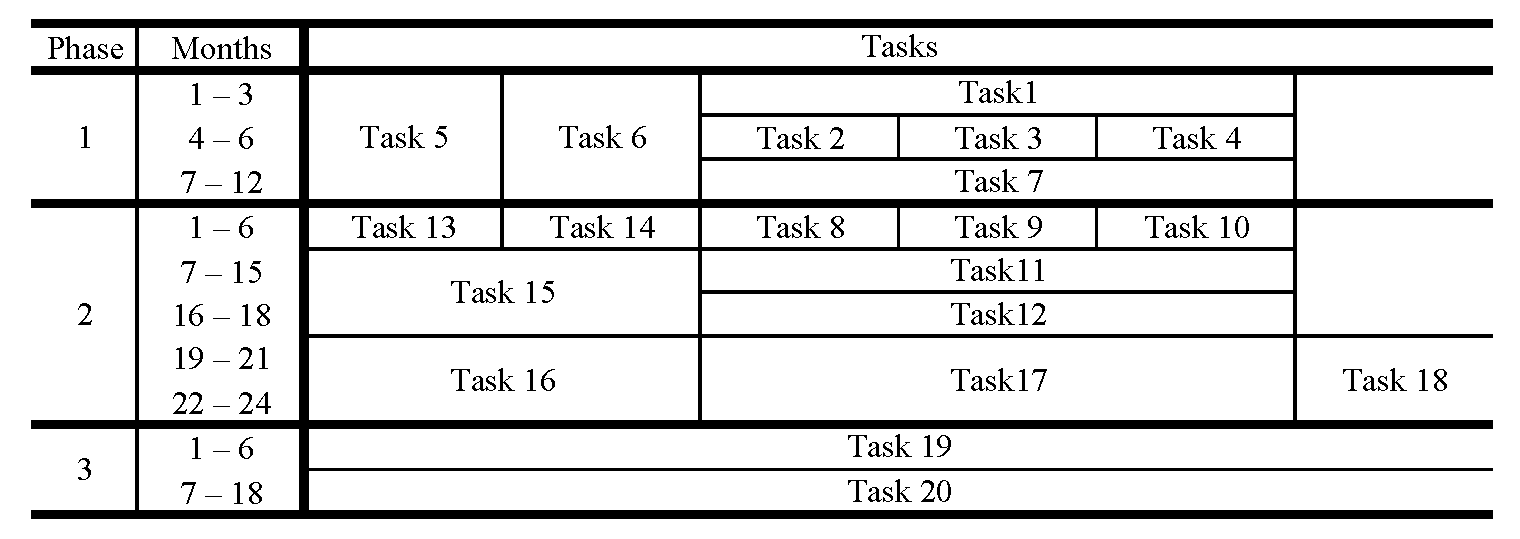
\includegraphics[width=1.0\linewidth]{fig/milestone.png}
\caption{Schedule and Milestone}
\label{tab:milestone}
\end{table}



\newpage
\section{Section III. Additional Information}
%\clearpage
%\pagenumbering{arabic}
%\def\thepage{F-\arabic{page}}
%% \bibliographystyle{numbersx}
\bibliographystyle{plain}
\bibliography{references,proposal,architecture2,architecture}

%\section{Summary Slide}
%\input{J-slide.tex}

\begin{comment}
%MURALI

Recent years have witnessed a rapid growth of computationally intensive applications on users' devices for military operations, such as image/video recognition for surveillance and autonomous navigation, augmented reality on mobile devices, and cyber security via real-time network log analysis of the users. These big data processing applications have been an exclusive domain of large enterprise class servers and datacenters. But in many of these application domains much of the data needed is collected at the edge devices such as sensors, mobile platforms. The data is then channelled through a collection of networked computation points to the backend servers. There is a significant amount of computing capability that is embedded along the entire path from edge to the cloud. Hence, exploiting these dispersed computing capabilities is not only beneficial for performance and power, but it is also required in the context of military operations, where uncertainty in available bandwidth and latency in decision making are critical considerations. In many scenarios access to the cloud can be very limited, or it may require significant backhaul data movement that is infeasible. As a result,  there is a critical need for enabling \emph{dispersed computing}, in which computation is carried out using the computational resources that are locally available to the users. 

\vspace{-0.1in}
\input{Task1.tex}
\vspace{-0.1in}
\input{Task2.tex}
\vspace{-0.1in}
\input{Task3.tex}

%\vspace{1em}
%\noindent {\LARGE \textbf{Phase 2}}
\vspace{-0.1in}
\input{Task4.tex}
\vspace{-0.1in}
\input{Task5.tex}
\vspace{-0.1in}
\input{Task6.tex}

\vspace{-0.1in}
\section{TA3 Integration Concept}
\label{sec:Integration}
\input{integration.tex}

\vspace{-0.1in}
\section{Management Plan}
\vspace{-0.1in}
The project requires expertise in distributed computing, online algorithms, communications, networking and runtime systems.  Towards that end, the proposed team consists of three prime members with the following expertise and unique capabilities:
\begin{itemize}[topsep=0pt,itemsep=0ex,partopsep=0ex,parsep=0ex,leftmargin=*]
\item \textbf{Dr. Salman Avestimehr (PI)} has expertise in distributed computing, coding, data analytics, network information theory, and communication networks. His major recent research accomplishment that is most relevant to this project is the invention of \emph{Coded Distributed Computing}~\cite{LMA_all,ComCom16,ComComJ16,EdgeCompG,EdgeCompACM} that provides a novel joint computing and communication design framework for distributed computing to significantly reduce the bandwidth consumption and response latency. 
\item \textbf{Dr. Murali Annavaram (co-PI)} is an expert in runtime systems for mobile computing, energy efficient computer system architecture, reliability and availability of high performance computing, and datacenter design.  His major recent research accomplishment that is most relevant to this project is a practical computational offloading system built on top of Android OS~\cite{lee2012wireless, annavaram2015runtime}, which was exclusively licensed to a major mobile device vendor for product adoption.
\item \textbf{Dr. Bhaskar Krishnamachari (co-PI)} has expertise in the design and analysis of algorithms and protocols for networked communication and computation, using tools from combinatorial algorithms, online learning, network utility optimization and game theory. His major  relevant accomplishments include the design of Hermes, the first $1+\epsilon$ approximation algorithm (FPTAS) for minimizing the latency (makespan) of scheduling the distributed computation for a large class of task graphs on an arbitrary network of processors~\cite{Hermes2015}, and LLR, the first polynomial-regret policy for online network optimization~\cite{Gai2012}. 
\end{itemize}


Dr. Avestimehr will be the principal investigator (PI) and responsible for overall project management. The three prime members are highly committed to collaborative research, and have already established a very effective and efficient collaborative environment. The task responsibilities of prime team members are shown in Table~\ref{table:roles}. There will also be one senior programmer, one postdoctoral scholar, and four PhD students involved in the project, with the following roles:
\begin{itemize}[topsep=0pt,itemsep=0ex,partopsep=0ex,parsep=0ex,leftmargin=*]
\item \textbf{Senior Research Programmer.} The senior research programmer (SRP) will assist in porting the coded optimization algorithms onto the two testbeds. SRP will be responsible for interacting with dispersive technologies to understand the system usage APIs and to port the algorithms developed by the PIs to match the testbed-specific needs. For the USC testbed, SRP will  be responsible for bringing up the Arduino and Raspberry Pi setups and interface them with appropriate sensors. SRP will setup the desktop computing infrastructure to enable appropriate RDMA, RoCE and RSCSI on the underlying hardware. SRP will also work with the graduate students and PIs to translate the code/data movement choices to use the right set of underlying interfaces and APIs in the heterogeneous testbeds.    
\item \textbf{Postdoctoral Scholar.} We will involve one postdoctoral scholar with expertise in distributed computing, resource allocation for computation workflows, and coding. The postdoctoral scholar will co-supervised by Dr. Avestimehr and Dr. Krishnamachari, and will facilitate collaborations between Tasks 1 and 2 in Phase 1, and Tasks 1 and 2 in Phase 2.
\item \textbf{PhD Students.} We will involve four PhD Student to work full time on this project. The first PhD student will focus on Task 1 in Phases 1 and 2, and will be supervised by Dr. Krishnamachari, the second PhD student will focus on Task 2 in Phases 1 and 2, and will be supervised by Dr. Avestimehr, the third PhD student will focus on Task 2 in Phases 1 and 2, and will be supervised by Dr. Annavaram, and the fourth PhD student will be co-supervised by Dr. Annavaram and Dr. Krishnamachari and collaborate on Tasks 1 and 3 in Phases 1 and 2, in order to facilitate interactions between these tasks. 
\end{itemize}
\begin{table}[t]
\vspace{-0.1in}
\begin{center}
    \begin{tabular}{|| p{4cm} ||  p{5cm} || p{6.4cm} ||}
    \hline
    \textbf{Prime Member} & \textbf{Leading Tasks} & \textbf{Collaborating Tasks}  \\ \hline
    Dr. Salman Avestimehr & {\small Overall project management, Phase 1 Task 2,  Phase 2 Task 2} & {\small Phase 1 Task 1, Phase 1 ST 3.4-3.6, Phase 2 Task 1,  Phase 2 ST 3.4-3.6}  \\ \hline
    Dr. Murali Annavaram &  {\small Phase 1 Task 3 \& Phase 2 Task 3} & {\small Interfaces with all tasks for testbed demo}  \\ \hline
    Dr. Bhaskar Krishnamachari & {\small Phase 1 Task 1 \& Phase 2 Task 1} & {\small Phase 1 Task 2, Phase 2 Task 2, Phase 1 ST 3.4-3.6, Phase 2 ST 3.4-3.6}  \\
    \hline
    \end{tabular}
    \end{center}
    \vspace{-0.2in}
    \caption{Task responsibilities of prime members.}
    \label{table:roles}
\end{table}



\noindent \textbf{Effort Coordination.} We will organize bi-weekly meetings in which all team member participate. The goal of the meeting will be to (1) discuss the new results obtained in the project, (2) identify new problems and research directions for collaboration, and (3) set the milestones for next meeting. We expect that at these meetings students will present an in-depth presentation of their current work and research progress to the entire group. To the extent possible our team will use existing open technological infrastructure such as github, trac and wikis to boost productivity. USC has extensive expertise in running open systems and will leverage these resources for this project. Our wiki site will be used initially for documenting the research progress internally, discussions on related work. The web site will serve as a repository for publications, annual program plans, quarterly progress reports, notes from meetings,  and all other products of research.
%We will organize bi-weekly meetings in which all team member participate. The goal of the meeting will be to (1) discuss the new results obtained in the project, (2) identify new problems and research directions for collaboration, and (3) set the milestones for next meeting.

\vspace{-0.2in}
\section{Personnel, Qualifications, and Commitments}
\vspace{-0.1in}
The proposed team consists of three prime members with the following qualifications and expertise:
\begin{itemize}[topsep=2pt,itemsep=-1ex,partopsep=1ex,parsep=1ex,leftmargin=*]
\item \textbf{Dr. Salman Avestimehr (PI)} is an Associate Professor at the Electrical Engineering Department of University of Southern California. Dr. Avestimehr has expertise in distributed computing, coding, data analytics, network information theory, and communication networks. His major recent research accomplishments include (1) invention of \emph{Coded Distributed Computing}~\cite{LMA_all,ComCom16,ComComJ16,EdgeCompG,EdgeCompACM} that provides a novel joint computing and communication design framework for distributed computing to significantly reduce the bandwidth consumption and response latency; (2) invention of \emph{Information-Theoretic Link Scheduling (ITLinQ)}~\cite{ITLinQJournal,ITLinQDyspan,ITLinQISIT,cachedITLinQ} that provides a new framework for spectrum sharing in device-to-device communication networks based on information-theoretic metrics, which significantly improves the state-of-the-art by increasing network throughput and fairness; and (3) development of new \emph{approximation techniques for network information theory}~\cite{DetMonograph,ADTJ09,MHMFMonograph,AASIT10} that allowed progress on decades-old open problems in network capacity. 

Dr. Avestimehr has received many awards for his research, including the Communications Society and Information Theory Society Joint Paper Award, the Presidential Early Career Award for Scientists and Engineers (PECASE) for ``pushing the frontiers of information theory through its extension to complex wireless information networks'', the Young Investigator Program (YIP) award from the U. S. Air Force Office of Scientific Research, and the National Science Foundation CAREER award. Dr. Avestimehr has led several large research projects, including a multi-university four-year research project on ``video-aware wireless networks'' and a multi-university four-year research project on ``Information Architectures for Femto-aided Networks''.

\item \textbf{Dr. Murali Annavaram (co-PI)} has seven years of industrial experience at Intel and Nokia prior to his appointment at USC. He designed and demonstrated physical prototypes and large scale testbeds, including the mobile century experiment where 100s of cars were equipped with mobile phones to generate traffic data using virtual trip lines~\cite{hoh2008virtual}. While working at Intel his research on Energy Per Instruction (EPI) throttling ~\cite{Annavaram2005}, formed the foundation for TurboBoost technology.  His work at Intel led to 8 issued/pending patents. He currently holds the Robert G. and Mary G. Lane Early Career Chair in the Ming-Hsieh Department of Electrical Engineering at the University of Southern California. Murali received NSF CAREER award in 2010 and an IBM Faculty Partnership award in 2009. Annavaram co-developed several hierarchical mobile sensing algorithms to improve energy efficiency of sensing platforms~\cite{wang2009-1,wang2009-2,wang2010,Liu2008}. Prior to his appointment at USC, he was a senior research scientist at the Intel Microprocessor Research Labs from 2001 to 2007 working on energy efficient server design and 3D stacking architectures. In 2007 he was a visiting researcher at  Nokia Research Center working on virtual trip line based traffic sensing. 

%His  recent research on improving mobile energy efficiency through dynamic computational offloading in the cloud has been exclusively licensed by a mobile manufacturer for commercialization.

\item \textbf{Dr. Bhaskar Krishnamachari (co-PI)} is a Professor and Ming Hsieh Faculty Fellow in Electrical Engineering with a joint appointment in Computer Science at the Viterbi School of Engineering, University of Southern California. He has expertise in the design and analysis of algorithms for next-generation networks, including distributed edge computing~\cite{Hermes, Latency14}, cognitive radio networks~\cite{GaiDSA14}, robotic networks~\cite{RouteSwarm}, connected vehicles~\cite{OptDissem, V2VCodedStorage}, and low power wireless embedded networks~\cite{BCP, MCC}. His work provides a bridge between theory and practice: developing and applying mathematical tools from combinatorial algorithms~\cite{GhoshGraph}, game theory~\cite{mm1, YWu16}, network utility maximization~\cite{Sridharan09}, stochastic decision theory~\cite{wang2010} and online learning~\cite{Gai2012} to practical problems in these domains. 

He has co-authored over 200 papers on these subjects, including several that have received best paper awards at ACM/IEEE IPSN (2004, 2010), ACM Mobicom (2010) and ACM MSWiM (2006), and collectively more than 19000 citations (per Google Scholar). He has also received the NSF Career Award (2004), the ASEE Terman Award (2010), and as listed in MIT Technology Review's TR-35 (2011), and Popular Science's Brilliant 10 (2015). He is the author of a textbook titled ``Networking Wireless Sensors" published by Cambridge University Press in 2005, and has served as an Associate Editor for the ACM Transactions on Sensor Networks, IEEE Transactions on Mobile Computing and IEEE Transactions on Wireless Communications. His research over the past decade and a half has been funded by Federal agencies including NSF, NASA, ARL, as well as industry sources including GM, Northrop Grumman, and Bosch Research. 

% During the course of this project, Krishnamachari is committed to spending significant time and effort (20\% of his time) on this project each year. He is not currently involved in any other large-scale funded research projects.

\end{itemize}

The level of effort in terms of hours to be expended by each person during each contract phase and other (current and proposed) major sources of support for each member with commitments of efforts for each source is shown in the table of Figure~\ref{fig:timeCommitment}.
\begin{figure}[t]
\vspace{-0.3in}
   \centering
   \includegraphics[width=0.75\textwidth]{timeCommitment.pdf}  
   \vspace{-0.2in}
   \caption{Time Commitments of Key Team Members}
   \label{fig:timeCommitment}
\end{figure}

\vspace{-0.1in}
\section{Capabilities}
\vspace{-0.1in}
\begin{itemize}[topsep=0pt,itemsep=0ex,partopsep=0ex,parsep=0ex,leftmargin=*]
\item Dr. Avestimehr, Annavaram, and Krishnamachari are directors of very successful research labs with outstanding PhD students, postdoctoral scholars, and MS students. They have expertise in distributed computing, online algorithms, communications, networking and runtime systems.
\item We maintain a 250 core high end compute cluster and five Nvidia GPU based systems for running distributed algorithms. However, these are not physically dispersed. We will rely on this cluster primarily for our initial debugging of distributed algorithms, and the final demonstrations will use the new dispersed testbeds. 
\item We maintain a 100-node Tutornet, a low power wireless embedded networking testbed that has been in operation since 2006 (http://anrg.usc.edu/www/tutornet/), and used by many researchers to evaluate algorithms and protocols for routing, transport, channel scheduling, resource allocation. This testbed will be federated with the new dispersed testbeds created during this project. 
\item We are in an excellent position to utilize a number of state of the art resources at the USC Viterbi School of Engineering, include the DETERLAB network security testbed at USC/ISI, and the USC High Performance Computing Center (HPCC).
\end{itemize} 

%Krishnamachari is the Director of the Autonomous Networks Research Group, consisting of 10 Ph.D. students at present (22 graduated to date), and also involving several MS and undergraduate students. His group maintains the 100-node Tutornet, a low power wireless embedded networking testbed that has been in operation since 2006 (http://anrg.usc.edu/www/tutornet/), and used by many researchers to evaluate algorithms and protocols for routing, transport, channel scheduling, resource allocation. This testbed will be federated with the new dispersed testbeds created during this project. 

\vspace{-0.2in}
\section{Statement of Work (SOW)}
\label{sec:sow}
\vspace{-0.1in}
\input{sow.tex}



\vspace{-0.1in}
\section{Schedule and Milestones}
\vspace{-0.1in}
The timeline of all tasks in the project, the interrelations among the tasks, and the milestones (i.e., demonstration plan) of the project are shown in Figure~\ref{fig:timelineALL}. There are a total of 9 demonstration plans and milestones during the project that are described in detail (with their corresponding goals, metrics, and deliverables) at the end of SOW (Section~\ref{sec:sow}).



\vspace{-0.1in}
\section{Level of Effort Summary by Task}
\vspace{-0.1in}
The estimated level of effort per task is summarized in the Table shown in Figure~\ref{fig:TaskHours}.

\begin{figure}[htp]
 \vspace{-2 mm}
   \centering
   \includegraphics[width=1\textwidth]{TaskHours2.pdf}
   \vspace{-0.3in}
   \caption{The estimated level of effort per task.}
   \label{fig:TaskHours}
 \vspace{-0.1in}
\end{figure}


\newpage
\section{Appendix A}

\begin{itemize}
\item \textbf{Team Member Identification:} The identification of team members is described in Table~\ref{table:teamID}.
\end{itemize}

\begin{table}[htp]
\begin{center}
    \begin{tabular}{|| l ||  l || p{4cm} || l | p{2cm} ||}
    \hline
    \textbf{Individual Name} & \textbf{Role} & \textbf{Organization} & \textbf{Non-US?} & \textbf{FFRDC or Govt?}  \\ \hline
    Dr. Salman Avestimehr & Prime & University of Southern California & No & None  \\ \hline
    Dr. Murali Annavaram & Prime & University of Southern California & No & None  \\ \hline
    Dr. Bhaskar Krishnamachari & Prime & University of Southern California & No & None  \\
    \hline
    \end{tabular}
    \end{center}
    \vspace{-0.2in}
    \caption{Task responsibilities of prime members.}
    \label{table:teamID}
\end{table}



\begin{itemize}
\item \textbf{Organizational Conflict of Interest Affirmations and Disclosure:} None.
\item \textbf{Intellectual Property (IP):} None.
\item \textbf{Human Subjects Research (HSR):} None.
\item \textbf{Animal Use:} None.
\end{itemize}

\begin{itemize}
\item \textbf{Representations Regarding Unpaid Delinquent Tax Liability or a Felony Conviction under Any Federal Law:}
\begin{enumerate}
    \item  The proposer is \textbf{not} a corporation that has any unpaid Federal tax liability that has been assessed, for which all judicial and administrative remedies have been exhausted or have lapsed, and that is not being paid in a timely manner pursuant to an agreement with the authority responsible for collecting the tax liability,
\item The proposer is \textbf{not} a corporation that was convicted of a felony criminal violation under a Federal law within the preceding 24 months.
\end{enumerate}
\item \textbf{Cost Accounting Standards (CAS) Notices and Certification:} None.
\end{itemize}

\newpage
\section{Appendix B}
%\clearpage
%\pagenumbering{arabic}
%\def\thepage{F-\arabic{page}}
%% \bibliographystyle{numbersx}
\bibliographystyle{IEEEbib}
\bibliography{bib/ref,bib/ref2,bib/salman,bib/salman1,bib/annavaram,bib/bk}
%\bibliography{bib/ref,bib/ref2,bib/salman,bib/salman1,bib/annavaram}

%\printbibliography
\end{comment}
\end{document}
